\documentclass[10pt,a4paper]{article}
% Build:  cd experiments/IMN && python -m experiments.IMN.code.latex_report  (tables, macros, figures)
%         cd report && latexmk -pdf report.tex
% Every number in this document is a macro from generated/macros.tex or a generated table (rule C2).
\usepackage[T1]{fontenc}
\usepackage{XCharter}
\usepackage[a4paper,margin=2.1cm]{geometry}
\usepackage{amsmath,amssymb}
\usepackage{booktabs,multirow,graphicx,subcaption,caption}
\usepackage[dvipsnames]{xcolor}
\usepackage{tikz}
\usetikzlibrary{positioning,arrows.meta,fit,backgrounds,calc,shapes.misc}
\usepackage{microtype,enumitem,placeins}
\usepackage[colorlinks,linkcolor=MidnightBlue,citecolor=MidnightBlue,urlcolor=MidnightBlue]{hyperref}
\captionsetup{font=small,labelfont=bf}
\setlist{nosep,leftmargin=*}

% generated by code/latex_report.py -- do not edit
\newcommand{\MainStatus}{complete}
\newcommand{\MainRecords}{720}
\newcommand{\MainDatasets}{12}
\newcommand{\MainSeeds}{5}
\newcommand{\MainimntmtmMean}{+0.0074}
\newcommand{\MainimntmtmLo}{+0.0038}
\newcommand{\MainimntmtmHi}{+0.0114}
\newcommand{\MainimntmtmWins}{11}
\newcommand{\MainimntmtmLosses}{1}
\newcommand{\MainimntmtmHolm}{0.024}
\newcommand{\MainimntmimnMean}{+0.0006}
\newcommand{\MainimntmimnLo}{-0.0140}
\newcommand{\MainimntmimnHi}{+0.0160}
\newcommand{\MainimntmimnWins}{6}
\newcommand{\MainimntmimnLosses}{6}
\newcommand{\MainimntmimnHolm}{1.000}
\newcommand{\MainimnhybridimnMean}{+0.0011}
\newcommand{\MainimnhybridimnLo}{-0.0134}
\newcommand{\MainimnhybridimnHi}{+0.0163}
\newcommand{\MainimnhybridimnWins}{6}
\newcommand{\MainimnhybridimnLosses}{6}
\newcommand{\MainimnhybridimnHolm}{1.000}
\newcommand{\MainimnhybridimntmMean}{+0.0005}
\newcommand{\MainimnhybridimntmLo}{-0.0004}
\newcommand{\MainimnhybridimntmHi}{+0.0014}
\newcommand{\MainimnhybridimntmWins}{9}
\newcommand{\MainimnhybridimntmLosses}{3}
\newcommand{\MainimnhybridimntmHolm}{1.000}
\newcommand{\MaintmgatedlrMean}{+0.0151}
\newcommand{\MaintmgatedlrLo}{-0.0158}
\newcommand{\MaintmgatedlrHi}{+0.0538}
\newcommand{\MaintmgatedlrWins}{7}
\newcommand{\MaintmgatedlrLosses}{5}
\newcommand{\MaintmgatedlrHolm}{1.000}
\newcommand{\MaintmgatedtmMean}{+0.0004}
\newcommand{\MaintmgatedtmLo}{-0.0090}
\newcommand{\MaintmgatedtmHi}{+0.0094}
\newcommand{\MaintmgatedtmWins}{8}
\newcommand{\MaintmgatedtmLosses}{4}
\newcommand{\MaintmgatedtmHolm}{1.000}
\newcommand{\MaintmgatedimnMean}{-0.0063}
\newcommand{\MaintmgatedimnLo}{-0.0250}
\newcommand{\MaintmgatedimnHi}{+0.0134}
\newcommand{\MaintmgatedimnWins}{7}
\newcommand{\MaintmgatedimnLosses}{5}
\newcommand{\MaintmgatedimnHolm}{1.000}
\newcommand{\MainimntmclauselrMean}{+0.0024}
\newcommand{\MainimntmclauselrLo}{+0.0002}
\newcommand{\MainimntmclauselrHi}{+0.0050}
\newcommand{\MainimntmclauselrWins}{9}
\newcommand{\MainimntmclauselrLosses}{3}
\newcommand{\MainimntmclauselrHolm}{0.879}
\newcommand{\MainimntmimntmrandMean}{-0.0009}
\newcommand{\MainimntmimntmrandLo}{-0.0061}
\newcommand{\MainimntmimntmrandHi}{+0.0049}
\newcommand{\MainimntmimntmrandWins}{5}
\newcommand{\MainimntmimntmrandLosses}{7}
\newcommand{\MainimntmimntmrandHolm}{1.000}
\newcommand{\MainimntabresnetMean}{+0.0026}
\newcommand{\MainimntabresnetLo}{-0.0004}
\newcommand{\MainimntabresnetHi}{+0.0061}
\newcommand{\MainimntabresnetWins}{9}
\newcommand{\MainimntabresnetLosses}{3}
\newcommand{\MainimntabresnetHolm}{0.831}
\newcommand{\MainFriedmanP}{\ensuremath{5.6\times 10^{-7}}}
\newcommand{\MainFriedmanChi}{50.3}
\newcommand{\MainCD}{4.81}
\newcommand{\MainRankN}{12}
\newcommand{\MainRanklr}{8.17}
\newcommand{\MainRankdt}{11.92}
\newcommand{\MainRankrf}{3.75}
\newcommand{\MainRankgbdt}{3.92}
\newcommand{\MainRanktabresnet}{6.33}
\newcommand{\MainRankimn}{5.83}
\newcommand{\MainRanktm}{8.50}
\newcommand{\MainRankclauselr}{6.50}
\newcommand{\MainRankimntm}{5.92}
\newcommand{\MainRankimntmrand}{5.00}
\newcommand{\MainRankimnhybrid}{5.50}
\newcommand{\MainRanktmgated}{6.67}
\newcommand{\MainGapCorr}{0.92}
\newcommand{\MainFidimn}{0.55}
\newcommand{\MainLinimn}{15}
\newcommand{\MainSelfimn}{0.65}
\newcommand{\MainFidclauselr}{0.74}
\newcommand{\MainClausesclauselr}{52}
\newcommand{\MainSelfclauselr}{1.00}
\newcommand{\MainFidimntm}{0.72}
\newcommand{\MainClausesimntm}{51}
\newcommand{\MainSelfimntm}{0.96}
\newcommand{\MainFidimntmrand}{0.54}
\newcommand{\MainClausesimntmrand}{40}
\newcommand{\MainSelfimntmrand}{0.69}
\newcommand{\MainFidimnhybrid}{0.73}
\newcommand{\MainClausesimnhybrid}{51}
\newcommand{\MainLinimnhybrid}{9}
\newcommand{\MainSelfimnhybrid}{0.97}
\newcommand{\MainFidtmgated}{0.45}
\newcommand{\MainLintmgated}{17}
\newcommand{\MainSelftmgated}{0.54}
\newcommand{\MainTimeimn}{41}
\newcommand{\MainTimeimntm}{42}
\newcommand{\MainTimetmgated}{16}
\newcommand{\MainTimetm}{3}
\newcommand{\MainWorstPaperGap}{phoneme (-0.068), jungle\_chess (-0.061)}
\newcommand{\HpoStatus}{complete}
\newcommand{\HpoRecords}{720}
\newcommand{\HpoDatasets}{12}
\newcommand{\HpoSeeds}{5}
\newcommand{\HpoimntmtmMean}{+0.0094}
\newcommand{\HpoimntmtmLo}{+0.0065}
\newcommand{\HpoimntmtmHi}{+0.0125}
\newcommand{\HpoimntmtmWins}{12}
\newcommand{\HpoimntmtmLosses}{0}
\newcommand{\HpoimntmtmHolm}{0.005}
\newcommand{\HpoimntmimnMean}{+0.0058}
\newcommand{\HpoimntmimnLo}{-0.0010}
\newcommand{\HpoimntmimnHi}{+0.0136}
\newcommand{\HpoimntmimnWins}{9}
\newcommand{\HpoimntmimnLosses}{3}
\newcommand{\HpoimntmimnHolm}{0.776}
\newcommand{\HpoimnhybridimnMean}{+0.0059}
\newcommand{\HpoimnhybridimnLo}{-0.0010}
\newcommand{\HpoimnhybridimnHi}{+0.0139}
\newcommand{\HpoimnhybridimnWins}{8}
\newcommand{\HpoimnhybridimnLosses}{4}
\newcommand{\HpoimnhybridimnHolm}{0.776}
\newcommand{\HpoimnhybridimntmMean}{+0.0001}
\newcommand{\HpoimnhybridimntmLo}{-0.0004}
\newcommand{\HpoimnhybridimntmHi}{+0.0006}
\newcommand{\HpoimnhybridimntmWins}{7}
\newcommand{\HpoimnhybridimntmLosses}{5}
\newcommand{\HpoimnhybridimntmHolm}{0.904}
\newcommand{\HpotmgatedlrMean}{+0.0254}
\newcommand{\HpotmgatedlrLo}{-0.0031}
\newcommand{\HpotmgatedlrHi}{+0.0629}
\newcommand{\HpotmgatedlrWins}{9}
\newcommand{\HpotmgatedlrLosses}{3}
\newcommand{\HpotmgatedlrHolm}{0.904}
\newcommand{\HpotmgatedtmMean}{+0.0049}
\newcommand{\HpotmgatedtmLo}{-0.0016}
\newcommand{\HpotmgatedtmHi}{+0.0096}
\newcommand{\HpotmgatedtmWins}{11}
\newcommand{\HpotmgatedtmLosses}{1}
\newcommand{\HpotmgatedtmHolm}{0.239}
\newcommand{\HpotmgatedimnMean}{+0.0013}
\newcommand{\HpotmgatedimnLo}{-0.0075}
\newcommand{\HpotmgatedimnHi}{+0.0116}
\newcommand{\HpotmgatedimnWins}{8}
\newcommand{\HpotmgatedimnLosses}{4}
\newcommand{\HpotmgatedimnHolm}{0.904}
\newcommand{\HpoimntmclauselrMean}{+0.0036}
\newcommand{\HpoimntmclauselrLo}{+0.0015}
\newcommand{\HpoimntmclauselrHi}{+0.0060}
\newcommand{\HpoimntmclauselrWins}{10}
\newcommand{\HpoimntmclauselrLosses}{2}
\newcommand{\HpoimntmclauselrHolm}{0.031}
\newcommand{\HpoimntmimntmrandMean}{+0.0007}
\newcommand{\HpoimntmimntmrandLo}{-0.0035}
\newcommand{\HpoimntmimntmrandHi}{+0.0037}
\newcommand{\HpoimntmimntmrandWins}{8}
\newcommand{\HpoimntmimntmrandLosses}{4}
\newcommand{\HpoimntmimntmrandHolm}{0.776}
\newcommand{\HpoimntabresnetMean}{-0.0061}
\newcommand{\HpoimntabresnetLo}{-0.0155}
\newcommand{\HpoimntabresnetHi}{-0.0001}
\newcommand{\HpoimntabresnetWins}{1}
\newcommand{\HpoimntabresnetLosses}{11}
\newcommand{\HpoimntabresnetHolm}{0.215}
\newcommand{\HpoFriedmanP}{\ensuremath{2.2\times 10^{-9}}}
\newcommand{\HpoFriedmanChi}{63.4}
\newcommand{\HpoCD}{4.81}
\newcommand{\HpoRankN}{12}
\newcommand{\HpoRanklr}{9.58}
\newcommand{\HpoRankdt}{11.42}
\newcommand{\HpoRankrf}{7.00}
\newcommand{\HpoRankgbdt}{3.75}
\newcommand{\HpoRanktabresnet}{4.50}
\newcommand{\HpoRankimn}{7.25}
\newcommand{\HpoRanktm}{9.08}
\newcommand{\HpoRankclauselr}{6.17}
\newcommand{\HpoRankimntm}{3.75}
\newcommand{\HpoRankimntmrand}{5.25}
\newcommand{\HpoRankimnhybrid}{3.92}
\newcommand{\HpoRanktmgated}{6.33}
\newcommand{\HpoGapCorr}{-0.11}
\newcommand{\HpoFidimn}{0.57}
\newcommand{\HpoLinimn}{16}
\newcommand{\HpoSelfimn}{0.72}
\newcommand{\HpoFidclauselr}{0.75}
\newcommand{\HpoClausesclauselr}{112}
\newcommand{\HpoSelfclauselr}{1.00}
\newcommand{\HpoFidimntm}{0.72}
\newcommand{\HpoClausesimntm}{126}
\newcommand{\HpoSelfimntm}{0.90}
\newcommand{\HpoFidimntmrand}{0.61}
\newcommand{\HpoClausesimntmrand}{115}
\newcommand{\HpoSelfimntmrand}{0.73}
\newcommand{\HpoFidimnhybrid}{0.69}
\newcommand{\HpoClausesimnhybrid}{121}
\newcommand{\HpoLinimnhybrid}{17}
\newcommand{\HpoSelfimnhybrid}{0.89}
\newcommand{\HpoFidtmgated}{0.47}
\newcommand{\HpoLintmgated}{19}
\newcommand{\HpoSelftmgated}{0.69}
\newcommand{\HpoTimeimn}{18}
\newcommand{\HpoTimeimntm}{25}
\newcommand{\HpoTimetmgated}{3}
\newcommand{\HpoTimetm}{6}
\newcommand{\TuneclauselrMean}{+0.0083}
\newcommand{\TuneclauselrWins}{11}
\newcommand{\TuneclauselrAuroc}{0.9035}
\newcommand{\DefaultclauselrAuroc}{0.8952}
\newcommand{\TunedtMean}{+0.0690}
\newcommand{\TunedtWins}{12}
\newcommand{\TunedtAuroc}{0.8611}
\newcommand{\DefaultdtAuroc}{0.7921}
\newcommand{\TunegbdtMean}{+0.0050}
\newcommand{\TunegbdtWins}{9}
\newcommand{\TunegbdtAuroc}{0.9066}
\newcommand{\DefaultgbdtAuroc}{0.9015}
\newcommand{\TuneimnMean}{+0.0043}
\newcommand{\TuneimnWins}{8}
\newcommand{\TuneimnAuroc}{0.9013}
\newcommand{\DefaultimnAuroc}{0.8970}
\newcommand{\TuneimnhybridMean}{+0.0091}
\newcommand{\TuneimnhybridWins}{10}
\newcommand{\TuneimnhybridAuroc}{0.9072}
\newcommand{\DefaultimnhybridAuroc}{0.8981}
\newcommand{\TuneimntmMean}{+0.0095}
\newcommand{\TuneimntmWins}{11}
\newcommand{\TuneimntmAuroc}{0.9071}
\newcommand{\DefaultimntmAuroc}{0.8976}
\newcommand{\TuneimntmrandMean}{+0.0079}
\newcommand{\TuneimntmrandWins}{9}
\newcommand{\TuneimntmrandAuroc}{0.9064}
\newcommand{\DefaultimntmrandAuroc}{0.8984}
\newcommand{\TunelrMean}{+0.0015}
\newcommand{\TunelrWins}{7}
\newcommand{\TunelrAuroc}{0.8771}
\newcommand{\DefaultlrAuroc}{0.8756}
\newcommand{\TunerfMean}{-0.0064}
\newcommand{\TunerfWins}{2}
\newcommand{\TunerfAuroc}{0.8962}
\newcommand{\DefaultrfAuroc}{0.9026}
\newcommand{\TunetabresnetMean}{+0.0131}
\newcommand{\TunetabresnetWins}{9}
\newcommand{\TunetabresnetAuroc}{0.9074}
\newcommand{\DefaulttabresnetAuroc}{0.8943}
\newcommand{\TunetmMean}{+0.0074}
\newcommand{\TunetmWins}{11}
\newcommand{\TunetmAuroc}{0.8976}
\newcommand{\DefaulttmAuroc}{0.8902}
\newcommand{\TunetmgatedMean}{+0.0119}
\newcommand{\TunetmgatedWins}{11}
\newcommand{\TunetmgatedAuroc}{0.9025}
\newcommand{\DefaulttmgatedAuroc}{0.8907}
\newcommand{\TuneimnWorst}{blood-transfusion (-0.073)}
\newcommand{\TuneimnBest}{jungle\_chess (+0.063), phoneme (+0.063)}
\newcommand{\TuneimntmWorst}{kc1 (-0.015)}
\newcommand{\TuneimntmBest}{jasmine (+0.024), credit-g (+0.023)}
\newcommand{\HpoImntmImnWorst}{vehicle (-0.017)}
\newcommand{\HpoImntmImnBest}{blood-transfusion (+0.037)}
\newcommand{\HpoImntmImnMeanNoBest}{+0.0029}
\newcommand{\TiertwoStatus}{complete}
\newcommand{\TiertwoRecords}{720}
\newcommand{\TiertwoDatasets}{20}
\newcommand{\TiertwoSeeds}{3}
\newcommand{\TiertwoimntmtmMean}{+0.0372}
\newcommand{\TiertwoimntmtmLo}{+0.0126}
\newcommand{\TiertwoimntmtmHi}{+0.0772}
\newcommand{\TiertwoimntmtmWins}{19}
\newcommand{\TiertwoimntmtmLosses}{1}
\newcommand{\TiertwoimntmtmHolm}{\ensuremath{9.5\times 10^{-5}}}
\newcommand{\TiertwoimntmimnMean}{+0.0183}
\newcommand{\TiertwoimntmimnLo}{+0.0072}
\newcommand{\TiertwoimntmimnHi}{+0.0314}
\newcommand{\TiertwoimntmimnWins}{15}
\newcommand{\TiertwoimntmimnLosses}{5}
\newcommand{\TiertwoimntmimnHolm}{0.030}
\newcommand{\TiertwoimnhybridimnMean}{+0.0185}
\newcommand{\TiertwoimnhybridimnLo}{+0.0071}
\newcommand{\TiertwoimnhybridimnHi}{+0.0319}
\newcommand{\TiertwoimnhybridimnWins}{15}
\newcommand{\TiertwoimnhybridimnLosses}{5}
\newcommand{\TiertwoimnhybridimnHolm}{0.025}
\newcommand{\TiertwoimnhybridimntmMean}{+0.0002}
\newcommand{\TiertwoimnhybridimntmLo}{-0.0011}
\newcommand{\TiertwoimnhybridimntmHi}{+0.0013}
\newcommand{\TiertwoimnhybridimntmWins}{14}
\newcommand{\TiertwoimnhybridimntmLosses}{6}
\newcommand{\TiertwoimnhybridimntmHolm}{0.350}
\newcommand{\TiertwotmgatedlrMean}{-0.0163}
\newcommand{\TiertwotmgatedlrLo}{-0.0354}
\newcommand{\TiertwotmgatedlrHi}{+0.0024}
\newcommand{\TiertwotmgatedlrWins}{6}
\newcommand{\TiertwotmgatedlrLosses}{14}
\newcommand{\TiertwotmgatedlrHolm}{0.359}
\newcommand{\TiertwotmgatedtmMean}{+0.0025}
\newcommand{\TiertwotmgatedtmLo}{-0.0271}
\newcommand{\TiertwotmgatedtmHi}{+0.0442}
\newcommand{\TiertwotmgatedtmWins}{7}
\newcommand{\TiertwotmgatedtmLosses}{13}
\newcommand{\TiertwotmgatedtmHolm}{0.883}
\newcommand{\TiertwotmgatedimnMean}{-0.0164}
\newcommand{\TiertwotmgatedimnLo}{-0.0359}
\newcommand{\TiertwotmgatedimnHi}{+0.0019}
\newcommand{\TiertwotmgatedimnWins}{5}
\newcommand{\TiertwotmgatedimnLosses}{15}
\newcommand{\TiertwotmgatedimnHolm}{0.350}
\newcommand{\TiertwoimntmclauselrMean}{+0.0141}
\newcommand{\TiertwoimntmclauselrLo}{-0.0035}
\newcommand{\TiertwoimntmclauselrHi}{+0.0470}
\newcommand{\TiertwoimntmclauselrWins}{7}
\newcommand{\TiertwoimntmclauselrLosses}{13}
\newcommand{\TiertwoimntmclauselrHolm}{0.883}
\newcommand{\TiertwoimntmimntmrandMean}{+0.0133}
\newcommand{\TiertwoimntmimntmrandLo}{+0.0058}
\newcommand{\TiertwoimntmimntmrandHi}{+0.0216}
\newcommand{\TiertwoimntmimntmrandWins}{16}
\newcommand{\TiertwoimntmimntmrandLosses}{4}
\newcommand{\TiertwoimntmimntmrandHolm}{0.005}
\newcommand{\TiertwoimntabresnetMean}{-0.0003}
\newcommand{\TiertwoimntabresnetLo}{-0.0069}
\newcommand{\TiertwoimntabresnetHi}{+0.0059}
\newcommand{\TiertwoimntabresnetWins}{7}
\newcommand{\TiertwoimntabresnetLosses}{13}
\newcommand{\TiertwoimntabresnetHolm}{0.883}
\newcommand{\TiertwoFriedmanP}{\ensuremath{9.4\times 10^{-20}}}
\newcommand{\TiertwoFriedmanChi}{116.4}
\newcommand{\TiertwoCD}{3.73}
\newcommand{\TiertwoRankN}{20}
\newcommand{\TiertwoRanklr}{7.60}
\newcommand{\TiertwoRankdt}{11.55}
\newcommand{\TiertwoRankrf}{3.10}
\newcommand{\TiertwoRankgbdt}{2.95}
\newcommand{\TiertwoRanktabresnet}{7.25}
\newcommand{\TiertwoRankimn}{7.65}
\newcommand{\TiertwoRanktm}{8.78}
\newcommand{\TiertwoRankclauselr}{4.00}
\newcommand{\TiertwoRankimntm}{4.95}
\newcommand{\TiertwoRankimntmrand}{6.80}
\newcommand{\TiertwoRankimnhybrid}{4.58}
\newcommand{\TiertwoRanktmgated}{8.80}
\newcommand{\TiertwoGapCorr}{0.67}
\newcommand{\TiertwoFidimn}{0.64}
\newcommand{\TiertwoLinimn}{257}
\newcommand{\TiertwoSelfimn}{0.92}
\newcommand{\TiertwoFidclauselr}{0.68}
\newcommand{\TiertwoClausesclauselr}{89}
\newcommand{\TiertwoSelfclauselr}{1.00}
\newcommand{\TiertwoFidimntm}{0.67}
\newcommand{\TiertwoClausesimntm}{85}
\newcommand{\TiertwoSelfimntm}{0.91}
\newcommand{\TiertwoFidimntmrand}{0.48}
\newcommand{\TiertwoClausesimntmrand}{150}
\newcommand{\TiertwoSelfimntmrand}{0.67}
\newcommand{\TiertwoFidimnhybrid}{0.71}
\newcommand{\TiertwoClausesimnhybrid}{87}
\newcommand{\TiertwoLinimnhybrid}{208}
\newcommand{\TiertwoSelfimnhybrid}{0.99}
\newcommand{\TiertwoFidtmgated}{0.52}
\newcommand{\TiertwoLintmgated}{251}
\newcommand{\TiertwoSelftmgated}{0.63}
\newcommand{\TiertwoTimeimn}{163}
\newcommand{\TiertwoTimeimntm}{166}
\newcommand{\TiertwoTimetmgated}{63}
\newcommand{\TiertwoTimetm}{37}
\newcommand{\TiertwoPaperGapCorr}{-0.88}
\newcommand{\TiertwoShortN}{6}
\newcommand{\TiertwoShortList}{higgs (-0.118), shuttle (-0.087), MiniBooNE (-0.077), KDDCup09\_appetency (-0.057), volkert (-0.052), jannis (-0.040)}
\newcommand{\TiertwoRestN}{14}
\newcommand{\TiertwoRestMean}{+0.0027}
\newcommand{\TiertwoRestWins}{9}
\newcommand{\TiertwoRestLosses}{5}
\newcommand{\TiertwoRestP}{0.194}
\newcommand{\TiertwoShortMean}{+0.0547}
\newcommand{\TiertwoCappedN}{15}
\newcommand{\TiertwoShortCapped}{6}
\newcommand{\RegMode}{prior}
\newcommand{\RegLambda}{1}
\newcommand{\RegValid}{0.8508}
\newcommand{\RegRecords}{324}
\newcommand{\Xaiimnlinear}{0.843}
\newcommand{\Xaiimnnonlinear}{0.541}
\newcommand{\Xaiimnpiecewise}{0.570}
\newcommand{\Xaiimntmlinear}{0.919}
\newcommand{\Xaiimntmnonlinear}{0.570}
\newcommand{\Xaiimntmpiecewise}{0.616}
\newcommand{\Xaitmgatedlinear}{0.736}
\newcommand{\Xaitmgatednonlinear}{0.400}
\newcommand{\Xaitmgatedpiecewise}{0.229}
\newcommand{\Xaigbdtlinear}{0.934}
\newcommand{\Xaigbdtnonlinear}{0.612}
\newcommand{\Xaigbdtpiecewise}{0.638}
\newcommand{\Xailrlinear}{0.975}
\newcommand{\XaiAuclrlinear}{0.997}
\newcommand{\Xailrnonlinear}{0.523}
\newcommand{\XaiAuclrnonlinear}{0.741}
\newcommand{\Xailrpiecewise}{0.576}
\newcommand{\XaiAuclrpiecewise}{0.757}
\newcommand{\Xaitabresnetlinear}{0.972}
\newcommand{\XaiAuctabresnetlinear}{0.997}
\newcommand{\Xaitabresnetnonlinear}{0.656}
\newcommand{\XaiAuctabresnetnonlinear}{0.970}
\newcommand{\Xaitabresnetpiecewise}{0.607}
\newcommand{\XaiAuctabresnetpiecewise}{0.847}
\newcommand{\XaiAucimnlinear}{0.997}
\newcommand{\XaiAucimnnonlinear}{0.968}
\newcommand{\XaiAucimnpiecewise}{0.848}
\newcommand{\XaiAucimntmlinear}{0.990}
\newcommand{\XaiAucimntmnonlinear}{0.974}
\newcommand{\XaiAucimntmpiecewise}{0.944}
\newcommand{\Xaitmlinear}{0.826}
\newcommand{\XaiAuctmlinear}{0.983}
\newcommand{\Xaitmnonlinear}{0.518}
\newcommand{\XaiAuctmnonlinear}{0.969}
\newcommand{\Xaitmpiecewise}{0.558}
\newcommand{\XaiAuctmpiecewise}{0.939}
\newcommand{\XaiVsimnMean}{+0.050}
\newcommand{\XaiVsimnWins}{41}
\newcommand{\XaiVsimnN}{60}
\newcommand{\XaiVsimnLosses}{19}
\newcommand{\XaiVsimnP}{\ensuremath{2.4\times 10^{-4}}}
\newcommand{\XaiVstmgatedMean}{+0.246}
\newcommand{\XaiVstmgatedWins}{59}
\newcommand{\XaiVstmgatedN}{60}
\newcommand{\XaiVstmgatedLosses}{1}
\newcommand{\XaiVstmgatedP}{\ensuremath{1.9\times 10^{-11}}}
\newcommand{\XaiVsgbdtMean}{-0.026}
\newcommand{\XaiVsgbdtWins}{10}
\newcommand{\XaiVsgbdtN}{60}
\newcommand{\XaiVsgbdtLosses}{50}
\newcommand{\XaiVsgbdtP}{\ensuremath{1.5\times 10^{-6}}}
\newcommand{\XaiLinDropimn}{-0.086}
\newcommand{\XaiLinDropimntm}{-0.003}
\newcommand{\XaiRecords}{540}
\newcommand{\AblTmFiftyMean}{-0.0034}
\newcommand{\AblTmFiftyWins}{7}
\newcommand{\AblTmFiftyLosses}{5}
\newcommand{\AblTmFiftyP}{0.733}
\newcommand{\AblTmFiftyVsImn}{--}
\newcommand{\AblTmFiftyFid}{--}
\newcommand{\AblTmFiftyRefFid}{--}
\newcommand{\AblTmEightMean}{+0.0036}
\newcommand{\AblTmEightWins}{9}
\newcommand{\AblTmEightLosses}{3}
\newcommand{\AblTmEightP}{0.077}
\newcommand{\AblTmEightVsImn}{--}
\newcommand{\AblTmEightFid}{--}
\newcommand{\AblTmEightRefFid}{--}
\newcommand{\AblImntmFiftyMean}{+0.0004}
\newcommand{\AblImntmFiftyWins}{6}
\newcommand{\AblImntmFiftyLosses}{6}
\newcommand{\AblImntmFiftyP}{0.850}
\newcommand{\AblImntmFiftyVsImn}{-0.0006}
\newcommand{\AblImntmFiftyFid}{0.71}
\newcommand{\AblImntmFiftyRefFid}{0.73}
\newcommand{\AblImntmEightMean}{-0.0012}
\newcommand{\AblImntmEightWins}{8}
\newcommand{\AblImntmEightLosses}{4}
\newcommand{\AblImntmEightP}{0.622}
\newcommand{\AblImntmEightVsImn}{-0.0021}
\newcommand{\AblImntmEightFid}{0.74}
\newcommand{\AblImntmEightRefFid}{0.73}
\newcommand{\AblNoinitMean}{+0.0002}
\newcommand{\AblNoinitWins}{6}
\newcommand{\AblNoinitLosses}{6}
\newcommand{\AblNoinitP}{0.970}
\newcommand{\AblNoinitVsImn}{-0.0007}
\newcommand{\AblNoinitFid}{0.65}
\newcommand{\AblNoinitRefFid}{0.73}
\newcommand{\AblXcMean}{-0.0116}
\newcommand{\AblXcWins}{5}
\newcommand{\AblXcLosses}{7}
\newcommand{\AblXcP}{0.064}
\newcommand{\AblXcVsImn}{-0.0126}
\newcommand{\AblXcFid}{0.71}
\newcommand{\AblXcRefFid}{0.73}
\newcommand{\AblRandfrMean}{-0.0017}
\newcommand{\AblRandfrWins}{8}
\newcommand{\AblRandfrLosses}{4}
\newcommand{\AblRandfrP}{0.850}
\newcommand{\AblRandfrVsImn}{-0.0026}
\newcommand{\AblRandfrFid}{0.56}
\newcommand{\AblRandfrRefFid}{0.73}
\newcommand{\AblSplitMean}{+0.0003}
\newcommand{\AblSplitWins}{8}
\newcommand{\AblSplitLosses}{4}
\newcommand{\AblSplitP}{0.339}
\newcommand{\AblSplitVsImn}{+0.0001}
\newcommand{\AblSplitFid}{0.74}
\newcommand{\AblSplitRefFid}{0.74}
\newcommand{\AblRecords}{288}
\newcommand{\TiertwoSkipped}{0}
\newcommand{\TiertwoSkippedList}{none}

% TikZ body of the graphical abstract; \input by graphical_abstract.tex (standalone) and report.tex.
% Needs: tikz with positioning, arrows.meta, fit, backgrounds, calc; the result macros.
\definecolor{gaInk}{HTML}{0B0B0B}
\definecolor{gaInkTwo}{HTML}{52514E}
\definecolor{gaMuted}{HTML}{8A8984}
\definecolor{gaGrid}{HTML}{E4E3DF}
\definecolor{gaBlue}{HTML}{2A78D6}
\definecolor{gaOrange}{HTML}{EB6834}
\definecolor{gaAqua}{HTML}{1BAF7A}
\definecolor{gaBox}{HTML}{3A3936}
\tikzset{
  ga/.style={font=\small, text=gaInk},
  ga panel/.style={draw=gaGrid, rounded corners=6pt, line width=0.8pt, fill=white},
  ga title/.style={font=\bfseries\normalsize, anchor=north west, text=gaInk},
  ga sub/.style={font=\footnotesize, text=gaInkTwo, anchor=north west},
  ga data/.style={draw=gaMuted, fill=gaGrid!40, rounded corners=2pt, minimum height=7mm, minimum width=13mm,
                  font=\footnotesize, align=center},
  ga black/.style={draw=gaBox, fill=gaBox, text=white, rounded corners=3pt, minimum height=9mm,
                   minimum width=27mm, font=\footnotesize, align=center},
  ga tm/.style={draw=gaOrange, fill=gaOrange!12, rounded corners=3pt, minimum height=9mm,
                minimum width=27mm, font=\footnotesize, align=center, line width=0.8pt},
  ga gen/.style={draw=gaAqua, fill=gaAqua!12, rounded corners=3pt, minimum height=9mm,
                 minimum width=27mm, font=\footnotesize, align=center, line width=0.8pt},
  ga local/.style={draw=#1, line width=1.1pt, rounded corners=3pt, fill=white, minimum height=10mm,
                   minimum width=44mm, font=\footnotesize, align=center},
  ga arrow/.style={-{Stealth[length=2.4mm]}, line width=0.9pt, draw=gaInkTwo},
  ga lbl/.style={font=\scriptsize, text=gaInkTwo, fill=white, inner sep=1pt},
  ga find/.style={draw=gaGrid, fill=gaGrid!35, rounded corners=4pt, text width=38.9mm, minimum height=17mm,
                  font=\scriptsize, align=left, inner sep=4pt, text=gaInk},
}
% a tiny table icon standing for the input row x
\newcommand{\gaTable}[1]{%
  \begin{scope}[shift={(#1)}]
    \foreach \i in {0,...,3} {\draw[gaMuted, fill=gaGrid!60] (\i*0.32,0) rectangle ++(0.30,0.30);}
  \end{scope}}
% horizontal impact bars: list of signed lengths
\newcommand{\gaBars}[3]{% anchor, colour, list
  \begin{scope}[shift={(#1)}]
    \draw[gaMuted, line width=0.5pt] (0,0.15) -- (0,-1.15);
    \foreach \v [count=\k] in {#3} {
      \fill[#2, rounded corners=0.6pt] (0,{-(\k-1)*0.26}) rectangle ({\v},{-(\k-1)*0.26-0.17});
    }
  \end{scope}}

\newcommand{\GraphicalAbstract}{%
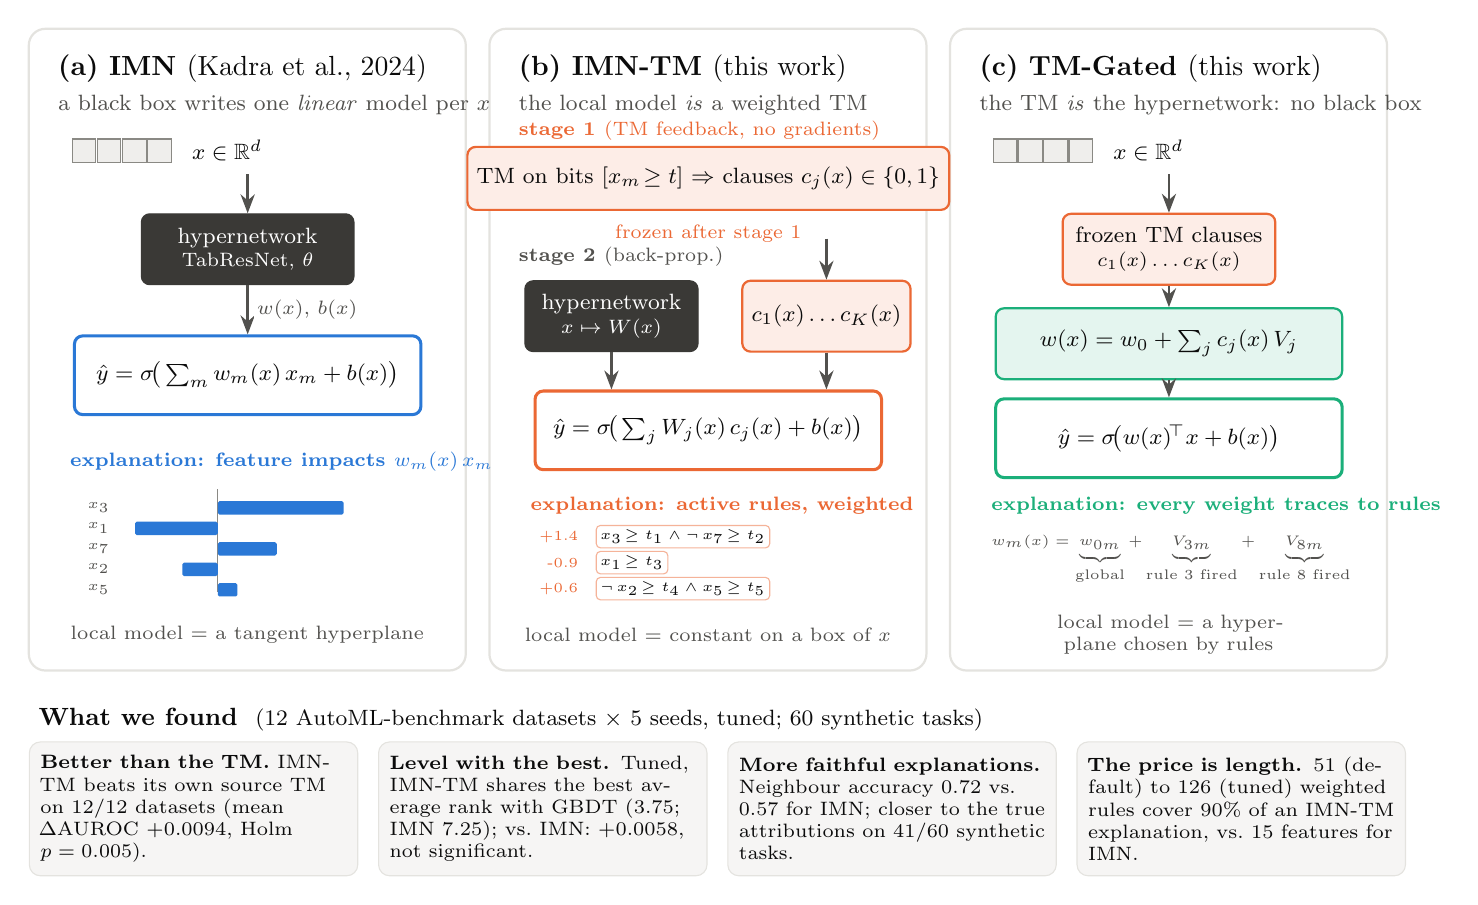
\begin{tikzpicture}[ga, x=1cm, y=1cm]
  % ---------------------------------------------------------------- panel geometry
  \def\pw{5.55} \def\ph{8.15} \def\gap{0.3}
  \foreach \p in {0,1,2} {\draw[ga panel] ({\p*(\pw+\gap)},0) rectangle ++(\pw,\ph);}

  % ================================================================= (a) IMN
  \begin{scope}[shift={(0,0)}]
    \node[ga title] at (0.25,\ph-0.2) {(a) IMN \textmd{(Kadra et al., 2024)}};
    \node[ga sub]   at (0.25,\ph-0.72) {a black box writes one \emph{linear} model per $x$};
    \gaTable{0.55,6.45}
    \node[font=\footnotesize, anchor=west] at (1.95,6.6) {$x\in\mathbb{R}^d$};
    \node[ga black] (hA) at (2.78,5.35) {hypernetwork\\[-1pt]{\scriptsize TabResNet, $\theta$}};
    \draw[ga arrow] (2.78,6.3) -- (hA.north);
    \node[ga local=gaBlue] (lA) at (2.78,3.75) {$\hat y=\sigma\!\big(\textstyle\sum_m w_m(x)\,x_m + b(x)\big)$};
    \draw[ga arrow] (hA.south) -- node[ga lbl, right=2pt] {$w(x),\,b(x)$} (lA.north);
    \node[font=\scriptsize\bfseries, text=gaBlue, anchor=west] at (0.4,2.65) {explanation: feature impacts $w_m(x)\,x_m$};
    \gaBars{2.4,2.15}{gaBlue}{1.6,-1.05,0.75,-0.45,0.25}
    \foreach \n [count=\k] in {$x_3$,$x_1$,$x_7$,$x_2$,$x_5$}
      \node[font=\tiny, text=gaInkTwo, anchor=east] at (1.15,{2.07-(\k-1)*0.26}) {\n};
    \node[font=\scriptsize, text=gaInkTwo, align=center, text width=5cm] at (\pw/2,0.45)
      {local model = a tangent hyperplane};
  \end{scope}

  % ================================================================= (b) IMN-TM
  \begin{scope}[shift={(\pw+\gap,0)}]
    \node[ga title] at (0.25,\ph-0.2) {(b) IMN-TM \textmd{(this work)}};
    \node[ga sub]   at (0.25,\ph-0.72) {the local model \emph{is} a weighted TM};
    % stage 1
    \node[font=\scriptsize\bfseries, text=gaOrange, anchor=west] at (0.25,6.85) {stage 1 \textmd{(TM feedback, no gradients)}};
    \node[ga tm, minimum width=46mm, minimum height=8mm] (tmB) at (2.78,6.25)
      {TM on bits $[x_m\!\ge t]$ $\Rightarrow$ clauses $c_j(x)\in\{0,1\}$};
    \node[font=\scriptsize, text=gaOrange, anchor=north] at (2.78,5.78) {frozen after stage 1};
    % stage 2
    \node[font=\scriptsize\bfseries, text=gaInkTwo, anchor=west] at (0.25,5.25) {stage 2 \textmd{(back-prop.)}};
    \node[ga black, minimum width=22mm] (hB) at (1.55,4.5) {hypernetwork\\[-1pt]{\scriptsize $x\mapsto W(x)$}};
    \node[ga tm, minimum width=19mm] (cB) at (4.28,4.5) {$c_1(x)\dots c_K(x)$};
    \draw[ga arrow] (tmB.south -| cB.north) ++(0,-0.35) -- (cB.north);
    \node[ga local=gaOrange] (lB) at (2.78,3.05) {$\hat y=\sigma\!\big(\textstyle\sum_j W_j(x)\,c_j(x) + b(x)\big)$};
    \draw[ga arrow] (hB.south) -- (hB.south |- lB.north);
    \draw[ga arrow] (cB.south) -- (cB.south |- lB.north);
    \node[font=\scriptsize\bfseries, text=gaOrange, anchor=west] at (0.4,2.1) {explanation: active rules, weighted};
    \foreach \w/\r [count=\k] in {+1.4/{$x_3\!\ge t_1 \wedge \neg\, x_7\!\ge t_2$},
                                  -0.9/{$x_1\!\ge t_3$},
                                  +0.6/{$\neg\, x_2\!\ge t_4 \wedge x_5\!\ge t_5$}} {
      \node[font=\tiny, anchor=east, text=gaOrange] at (1.25,{1.7-(\k-1)*0.33}) {\w};
      \node[font=\tiny, anchor=west, draw=gaOrange!50, rounded corners=1.5pt, inner sep=1.5pt]
        at (1.35,{1.7-(\k-1)*0.33}) {\r};
    }
    \node[font=\scriptsize, text=gaInkTwo, align=center, text width=5cm] at (\pw/2,0.45)
      {local model = constant on a box of $x$};
  \end{scope}

  % ================================================================= (c) TM-Gated
  \begin{scope}[shift={(2*\pw+2*\gap,0)}]
    \node[ga title] at (0.25,\ph-0.2) {(c) TM-Gated \textmd{(this work)}};
    \node[ga sub]   at (0.25,\ph-0.72) {the TM \emph{is} the hypernetwork: no black box};
    \gaTable{0.55,6.45}
    \node[font=\footnotesize, anchor=west] at (1.95,6.6) {$x\in\mathbb{R}^d$};
    \node[ga tm] (cC) at (2.78,5.35) {frozen TM clauses\\[-1pt]{\scriptsize $c_1(x)\dots c_K(x)$}};
    \draw[ga arrow] (2.78,6.3) -- (cC.north);
    \node[ga gen, minimum width=44mm] (gC) at (2.78,4.15) {$w(x)=w_0+\textstyle\sum_j c_j(x)\,V_j$};
    \draw[ga arrow] (cC.south) -- (gC.north);
    \node[ga local=gaAqua] (lC) at (2.78,2.95) {$\hat y=\sigma\!\big(w(x)^{\!\top} x + b(x)\big)$};
    \draw[ga arrow] (gC.south) -- (lC.north);
    \node[font=\scriptsize\bfseries, text=gaAqua, anchor=west] at (0.4,2.1) {explanation: every weight traces to rules};
    \node[font=\tiny, text=gaInkTwo, align=left, anchor=north west, text width=4.9cm] at (0.4,1.85)
      {$w_m(x) = \underbrace{w_{0m}}_{\text{global}} + \underbrace{V_{3m}}_{\text{rule 3 fired}} + \underbrace{V_{8m}}_{\text{rule 8 fired}}$};
    \node[font=\scriptsize, text=gaInkTwo, align=center, text width=5cm] at (\pw/2,0.45)
      {local model = a hyperplane chosen by rules};
  \end{scope}

  % ================================================================= findings strip
  \def\fy{-0.35}
  \node[font=\bfseries\small, anchor=north west] at (0,\fy) {What we found
    \textmd{\footnotesize\ (\HpoDatasets\ AutoML-benchmark datasets $\times$ \HpoSeeds\ seeds, tuned; \XaiVsimnN\ synthetic tasks)}};
  \node[ga find, anchor=north west] (f1) at (0,\fy-0.55)
    {\textbf{Better than the TM.} IMN-TM beats its own source TM on \HpoimntmtmWins/\HpoDatasets\ datasets
     (mean $\Delta$AUROC \HpoimntmtmMean, Holm $p=\HpoimntmtmHolm$).};
  \node[ga find, right=2.5mm of f1] (f2)
    {\textbf{Level with the best.} Tuned, IMN-TM shares the best average rank with GBDT
     (\HpoRankimntm; IMN \HpoRankimn); vs.\ IMN: \HpoimntmimnMean, not significant.};
  \node[ga find, right=2.5mm of f2] (f3)
    {\textbf{More faithful explanations.} Neighbour accuracy \HpoFidimntm\ vs.\ \HpoFidimn\ for IMN; closer to
     the true attributions on \XaiVsimnWins/\XaiVsimnN\ synthetic tasks.};
  \node[ga find, right=2.5mm of f3] (f4)
    {\textbf{The price is length.} \MainClausesimntm\ (default) to \HpoClausesimntm\ (tuned) weighted rules
     cover 90\% of an IMN-TM explanation, vs.\ \MainLinimn\ features for IMN.};
\end{tikzpicture}}

\newcommand{\imn}{\textsc{IMN}}
\newcommand{\arm}[1]{\textsf{#1}}

\title{Replacing the Linear Local Model of Interpretable Mesomorphic Networks\\with a Tsetlin Machine}
\author{IMN $\times$ TM research programme, \texttt{experiments/IMN} \\
  \small torchtsetlin 0.3.1, revision \texttt{06a2ce5}}
\date{\today}

\begin{document}
\maketitle

\begin{abstract}
Interpretable Mesomorphic Networks (\imn{}; Kadra et al., NeurIPS 2024) train a deep hypernetwork that
writes, for every example, a linear model in the original feature space; the linear model is both the
prediction and its explanation. Their stated limitation is that the per-example models are linear. We
replace the linear model by a \emph{Tsetlin machine} (TM), a weighted vote of conjunctive rules over
thresholded features. Because TM clauses are learned by discrete feedback and have no gradient, we train a
TM first, freeze its clauses, and let the hypernetwork generate per-example \emph{clause weights}
(\arm{IMN-TM}); we also study a linear+rules hybrid and a model in which the TM itself plays the
hypernetwork (\arm{TM-Gated}, no black box).

\emph{Accuracy.} On \MainDatasets{} AutoML-benchmark datasets with default hyper-parameters
(\MainRecords{} runs), \arm{IMN-TM} improves on its source TM on
\MainimntmtmWins/\MainDatasets{} datasets (Holm $p=\MainimntmtmHolm$) and ties \imn{} on average
($\Delta$AUROC \MainimntmimnMean). The per-dataset difference tracks how much tree ensembles beat
linear models (Pearson $r=\MainGapCorr$). After a 20-trial search per method (\HpoRecords{}
final runs), \arm{IMN-TM} beats its TM on \HpoimntmtmWins/\HpoDatasets{} datasets and a global
re-fit of its clause weights (Holm $p=\HpoimntmclauselrHolm$). It shares the best average rank
with gradient boosting (\HpoRankimntm), ahead of \imn{} (\HpoRankimn). Its margin over \imn{}
(\HpoimntmimnMean) is not significant, and the tree-gap pattern disappears because tuning
mostly helps \imn{} on threshold-shaped data.

\emph{Explanations.} Clause explanations remain valid on an example's neighbourhood: local
fidelity is \HpoFidimntm{} vs.\ \HpoFidimn{} for \imn{}. On \XaiVsimnN{} synthetic tasks with
known contributions, they are closer to the truth than \imn{}'s on \XaiVsimnWins{} tasks
(Wilcoxon $p=\XaiVsimnP$). The price is length: \MainClausesimntm--\HpoClausesimntm{} weighted
rules vs.\ \MainLinimn{} features cover 90\% of an explanation.

\emph{Larger datasets.} On \TiertwoDatasets{} larger datasets under a fixed training budget,
\arm{IMN-TM} beats \imn{} significantly (\TiertwoimntmimnMean, Holm $p=\TiertwoimntmimnHolm$).
The gain comes almost entirely from datasets where the step cap leaves \imn{} under-trained
($r=\TiertwoPaperGapCorr$ with \imn{}'s shortfall against the paper); elsewhere it is
\TiertwoRestMean.

\emph{What matters.} Ablations show that learned clauses matter for explanation fidelity, not
for accuracy, and that initialising at the TM's votes matters for fidelity and for
budget-limited training.
\end{abstract}

\begin{figure}[t]
  \centering
  \resizebox{\textwidth}{!}{\GraphicalAbstract}
  \caption{\textbf{Graphical abstract.} (a) \imn{}: a TabResNet hypernetwork generates a linear model per
  example. (b) \arm{IMN-TM}: a Tsetlin machine is trained first (stage 1) and its clauses are frozen; the
  hypernetwork then generates one weight per clause and example (stage 2), so the local model is a weighted
  TM. (c) \arm{TM-Gated}: the frozen clauses themselves generate the coefficients of a linear model, so no
  black box remains. Rules in (b) and coefficients in (c) are schematic; Figure~\ref{fig:example} shows a
  real explanation. Findings: tuned hyper-parameters, \HpoDatasets{} datasets $\times$ \HpoSeeds{} seeds, and the synthetic benchmark of Section~\ref{sec:xai}.}
  \label{fig:ga}
\end{figure}

\section{Introduction}
\imn{} \cite{kadra2024} make a deep tabular model explainable by construction: a hypernetwork
$w(x;\theta)$ outputs the parameters of a linear model, and the logit is that linear model evaluated at
$x$, $z_k(x)=\sum_m w_{km}(x)\,x_m + w_{k0}(x)$. The explanation of $x$ is the vector of feature impacts
$w_m(x)\,x_m$. Section~7 of the paper names the obvious limitation: the local models are hyperplanes, and
it suggests non-linear interpretable local models as future work.

A Tsetlin machine \cite{granmo2018} is an interpretable non-linear model of exactly that kind: a weighted
sum of conjunctions (\emph{clauses}) of Boolean literals, $v_k(x)=\sum_j W_{kj}\,c_j(x)$, where on tabular
data each literal is a threshold test $x_m\ge t$ or its negation. This report asks whether the linear
local model of \imn{} can be replaced by a TM, what that costs in accuracy, and what it changes about the
explanations. Contributions:
\begin{enumerate}
  \item a feasibility analysis and three constructions (Section~\ref{sec:method}), implemented on top of
        the \texttt{torchtsetlin} library without modifying it;
  \item a faithful re-implementation of \imn{} (read from the official code) and a controlled comparison
        with the original TM, \imn{} and the paper's baselines on the AutoML benchmark, with default and
        equal-budget tuned hyper-parameters;
  \item interpretability measurements that apply to every method: removal attributions, explanation
        size, local fidelity, self-consistency, and ground-truth attribution quality on synthetic tasks.
\end{enumerate}

\section{Method}\label{sec:method}
Readers who prefer numbers to symbols can start with Section~\ref{sec:example}. It follows one
toy example through every equation of this section.

\subsection{Why the clauses must be frozen}
A hypernetwork is trained by back-propagation, so whatever it generates must enter the loss
differentiably. A TM clause is a discrete set of included literals learned by Type~I/II feedback; it has
no gradient. The clause \emph{weights}, however, are continuous, and once the clauses are fixed their
outputs $c_j(x)\in\{0,1\}$ are ordinary Boolean features of $x$. This gives three constructions
(Figure~\ref{fig:ga}); a fourth---a hypernetwork that emits the clauses themselves---is not pursued: the
include masks are discrete, and a rule generated \emph{for} $x$ and evaluated \emph{at} $x$ is trivially
true or false, so it explains nothing unless constrained to a neighbourhood.

\paragraph{IMN-TM (local model = weighted TM).} With a frozen clause basis $c(x)\in\{0,1\}^K$ from a TM
trained in stage~1, the hypernetwork outputs $W(x)\in\mathbb{R}^{K\times n_\text{out}}$ and $b(x)$, and
\begin{equation}
  z_k(x)=\sum_{j=1}^{K} W_{kj}(x)\,c_j(x)+b_k(x).\label{eq:imntm}
\end{equation}
The output layer is zero-initialised and its bias set to the TM's signed clause votes divided by $T$, so
before training \arm{IMN-TM} \emph{is} the source TM (unclamped), for every input. The explanation is the
list of active rules with their weights $W_{kj}(x)$.

\paragraph{IMN-Hybrid.} The local model has both terms, $z_k(x)=\sum_m w_{km}(x)x_m+\sum_j W_{kj}(x)c_j(x)+b_k(x)$.

\paragraph{TM-Gated (TM as the hypernetwork).} The local model stays linear, but its coefficients are a
linear function of the clause outputs, $w_k(x)=w_{0k}+\sum_j c_j(x)\,V_{jk}$, learned by gradient descent
with the clauses frozen. Every coefficient of every local model is a global term plus one term per fired
rule, so the whole model is interpretable.

\paragraph{Controls.} \arm{Clause-LR} re-fits one \emph{global} weight per clause (no hypernetwork);
\arm{IMN-TM (rand.)} replaces the learned clauses by random data-anchored conjunctions of matched length.

\subsection{Training and regularisation}
Stage~1 trains a weighted TM (\texttt{torchtsetlin}, 200 clauses per class, $T=100$, $s=5$, batch
feedback with batch 32) on a thermometer encoding with up to 10 unique quantile thresholds per
standardised column, keeping the validation-best epoch. Duplicate and empty clauses are removed. Stage~2
reproduces the official \imn{} training loop exactly: TabResNet with 2 blocks of width 128, Adam with
learning rate and weight decay 0.01, 5 warm-up epochs, cosine annealing with three warm restarts, three
snapshots, 500 epochs, batch 64, and an $\ell_1$ penalty $\lambda\,\overline{|w(x)|}$ on the generated
parameters. For the clause arms the penalty can instead shrink the generated weights toward the TM's votes,
$\lambda\,\overline{|W(x)-W_\text{TM}|}$ (\texttt{prior}); Section~\ref{sec:reg} selects between the variants on
validation data.

\subsection{Attribution for every method}
Following Eq.~(2) of the paper, the impact of feature $m$ is the change of the explained logit when $x_m$
is set to 0 (its training mean) \emph{with the local model held fixed}:
$\phi_m(x)=z(x;w(x))-z(x\odot\delta^m;w(x))$. For \imn{} this is exactly $w_m(x)x_m$ (tested); for clause
local models the clauses are re-evaluated on the modified input; methods without a local model use the same
removal on the full model (occlusion).

% Worked example of the method (Section 2.4). The toy numbers are illustrative, chosen by hand and
% checked by hand-written arithmetic; they are not results and do not come from results/*.json.
\subsection{A worked example}\label{sec:example}
This section follows one toy input through every step of \arm{IMN-TM}, then through \imn{} and
\arm{TM-Gated}, so that each symbol in the equations above has a concrete value. The numbers are
\emph{illustrative}: they are chosen by hand to be easy to follow and are not measured. A real run
differs only in size. It has tens to thousands of threshold bits, hundreds of clauses, $T=100$
instead of $T=10$, and weights produced by a trained TabResNet. Table~\ref{tab:notation} collects
the notation and Figure~\ref{fig:worked} draws the whole computation.

\paragraph{The task.} A binary task ($y=1$: disease, $y=0$: healthy) with $d=2$ numeric features, \emph{age} and
\emph{blood pressure} (bp). As in the official \imn{} pipeline, numeric columns are standardised on the
training split, so a value is in units of standard deviations from the training mean. The example to
explain is
\[
  x=(x_1,x_2)=(\underbrace{0.8}_{\text{age}},\ \underbrace{-0.3}_{\text{bp}}),\qquad y=1 ,
\]
a somewhat older patient with slightly low blood pressure. Binary tasks use a single output
($n_\text{out}=1$), so the model produces one logit $z(x)$ and $p(y{=}1\mid x)=\sigma(z(x))$.

\begin{table}[h!]
  \centering\small\setlength{\tabcolsep}{4pt}
  \caption{Notation, with the value each symbol takes in the worked example of Section~\ref{sec:example}.}
  \label{tab:notation}
  \begin{tabular}{@{}l l l l@{}}
    \toprule
    Symbol & Meaning & Shape & Toy value\\
    \midrule
    $x=(x_1,\dots,x_d)$ & standardised input features & $d$ & $(0.8,\,-0.3)$, $d=2$\\
    $t_b,\ m(b)$ & threshold of bit $b$ and the feature it reads & per bit & $t_2=0.2$, $m(2)=1$ (age)\\
    $\beta_b(x)=[x_{m(b)}\ge t_b]$ & Boolean (thermometer) bit & $F$ bits & $(1,1,0,\,1,0,0)$, $F=6$\\
    $\ell(x)=(\beta,\ \lnot\beta)$ & literals: every bit and its negation & $2F$ & 12 literals\\
    $c_j(x)$ & output of clause $j$ (AND of its literals) & $K$ & $(1,0,1)$, $K=3$\\
    $W^\text{TM}_{j}$ & signed integer vote of clause $j$ in the trained TM & $K\times n_\text{out}$ & $(+6,\,+4,\,-3)$\\
    $T$ & TM vote margin (scales votes to logits) & scalar & $10$ (real runs: $100$)\\
    $W_{j}(x),\ b(x)$ & clause weights and bias generated for $x$ & $K\times n_\text{out}$, $n_\text{out}$ & $(1.4,\,0.2,\,-0.5)$, $-0.3$\\
    $z(x)$ & logit of the local model & $n_\text{out}$ & $0.6$\\
    $\lambda$ & strength of the penalty on generated weights & scalar & $0.1$\\
    $\phi_m(x)$ & removal attribution of feature $m$ & $d$ & $(1.4,\,-0.2)$\\
    \bottomrule
  \end{tabular}
\end{table}

\paragraph{Step 1: from numbers to bits.} The TM reads Boolean inputs, so every feature is cut at a few
thresholds (\emph{thermometer} encoding). The thresholds are quantiles of the training data; real runs
keep up to 10 per feature, and the toy keeps 3:
\[
\begin{array}{l@{\qquad}ccc@{\qquad}l}
  \text{age } (x_1=0.8): & t_1=-0.5 & t_2=0.2 & t_3=0.9 & \beta_{1..3}=(1,1,0)\\
  \text{bp } (x_2=-0.3): & t_4=-0.6 & t_5=0.0 & t_6=0.7 & \beta_{4..6}=(1,0,0)
\end{array}
\qquad \beta_b(x)=[\,x_{m(b)}\ge t_b\,].
\]
Here $[\cdot]$ is 1 when the condition holds and 0 otherwise, and $m(b)$ is the feature that bit $b$
reads. Bits 1--3 have $m(b)=1$ (age) and bits 4--6 have $m(b)=2$ (bp). The thermometer pattern
$1,1,0$ says ``age is at least $0.2$ but below $0.9$''. The TM may use each bit as it is or negated,
which gives $2F=12$ literals $\ell(x)$.

\paragraph{Step 2: the frozen clauses (stage 1).} A weighted TM is trained on the bits as usual. After
training, its clauses are fixed rules. Suppose that, once empty and duplicate clauses are removed,
$K=3$ remain:
\[
\begin{array}{l@{\ \ }l@{\qquad}c@{\qquad}r}
  & \text{clause (in words)} & c_j(x) & W^\text{TM}_j\\[2pt]
  c_1: & [\text{age}\ge0.2]\ \land\ \lnot[\text{bp}\ge0.7] & 1\land1=1 & +6\\
  c_2: & [\text{bp}\ge0.0]                               & 0          & +4\\
  c_3: & \lnot[\text{age}\ge0.9]\ \land\ [\text{bp}\ge-0.6] & 1\land1=1 & -3
\end{array}
\]
A clause outputs 1 only when \emph{all} of its literals are 1. For a binary task, $W^\text{TM}_j$ is the
clause's vote for class~1 minus its vote for class~0: $c_1$ and $c_2$ vote for disease, and $c_3$ votes
for healthy. The TM's own prediction is the vote sum scaled by the margin $T$:
\[
  z^\text{TM}(x)=\frac{1}{T}\sum_{j=1}^{K}W^\text{TM}_j\,c_j(x)=\frac{6\cdot1+4\cdot0-3\cdot1}{10}=0.3,
  \qquad \sigma(0.3)=0.57 .
\]
The weights $W^\text{TM}_j$ are the \emph{same for every patient}, which makes the TM a global model. From
here on the clauses never change. For any input, $c(x)\in\{0,1\}^K$ is just a vector of $K$ yes/no
answers, and gradient descent can use it like any other fixed feature.

\paragraph{Step 3: the hypernetwork writes a local model (stage 2).} The TabResNet hypernetwork reads the
\emph{raw} standardised input $x=(0.8,-0.3)$ and outputs $P=K+1=4$ numbers: one weight per clause and a
bias. For a $C$-class task it outputs $(K{+}1)\times C$ numbers. Suppose that for this patient it
outputs
\[
  W(x)=(W_1(x),W_2(x),W_3(x))=(1.4,\ 0.2,\ -0.5),\qquad b(x)=-0.3 .
\]
The local model is the TM with these weights in place of $W^\text{TM}/T$. This is Eq.~\eqref{eq:imntm} with
$n_\text{out}=1$:
\[
  z(x)=\sum_{j=1}^{K}W_j(x)\,c_j(x)+b(x)=1.4\cdot1+0.2\cdot0-0.5\cdot1-0.3=0.6,\qquad \sigma(0.6)=0.65 .
\]
Only \emph{active} clauses ($c_j(x)=1$) contribute. $W_2(x)=0.2$ is generated, but it is multiplied by
$c_2(x)=0$ and is not part of the explanation. The explanation of this prediction reads: ``\emph{age
$\ge0.2$ and bp $<0.7$} pushes towards disease with weight $1.4$; \emph{age $<0.9$ and bp $\ge-0.6$}
pushes towards healthy with weight $0.5$; baseline $-0.3$.'' Each rule is a box in feature space.

Another patient gets other weights. For $x'=(-0.9,\,0.8)$ the bits are $(0,0,0,\,1,1,1)$ and the active
clauses are $c(x')=(0,1,1)$. If the hypernetwork outputs $W(x')=(0.9,1.1,-0.2)$ and $b(x')=0.1$, then
$z(x')=1.1-0.2+0.1=1.0$. This explanation is led by the rule ``\emph{bp $\ge0$}'' with weight $1.1$. The
global TM, by contrast, gives that rule $4/10=0.4$ for every patient. \emph{Which rules count, and by
how much, is decided per example; what the rules are is decided once, by the TM.}

\paragraph{Step 4: initialisation at the TM.} Before training, the last layer of the hypernetwork is
zero. Its bias is set to $W^\text{TM}/T=(0.6,0.4,-0.3)$ for the clause weights and to $0$ for $b$. The
hypernetwork therefore outputs exactly these numbers for every input, and the untrained \arm{IMN-TM}
reproduces the TM: $z(x)=0.6\cdot1+0.4\cdot0-0.3\cdot1+0=0.3=z^\text{TM}(x)$. Training then only
\emph{moves} the weights away from the TM's votes where that lowers the loss. The one difference from
the TM is that the TM clamps each class's vote sum to $[-T,T]$, and this initialisation does not.

\paragraph{Step 5: the training loss.} The hypernetwork parameters $\theta$ are trained by Adam on the
cross-entropy plus a penalty on the generated parameters. For the \texttt{prior} variant the penalty
pulls them towards the TM initialisation $w^\text{prior}=(0.6,0.4,-0.3,\,0)$:
\[
  \mathcal{L}(x,y)=\underbrace{-\log\sigma(z(x))}_{y=1:\ \log(1+e^{-0.6})=0.437}
  +\ \lambda\,\underbrace{\tfrac{1}{P}\textstyle\sum_{p=1}^{P}\big|w_p(x)-w^\text{prior}_p\big|}_{(0.8+0.2+0.2+0.3)/4=0.375}
  =0.437+0.1\cdot0.375=0.475 .
\]
Here $w(x)=(W(x),b(x))$ is the full generated vector of length $P$, and $\lambda=0.1$ is an example
value. The gradient of $\mathcal{L}$ flows through $z(x)$ into $W(x)$ and $b(x)$, and from there into
$\theta$. It never flows into the clauses, which is why they had to be learned first. With the original
\texttt{all} variant, $w^\text{prior}=0$ and the penalty is $\lambda\,\overline{|w(x)|}$ as in \imn{}.

\paragraph{Step 6: feature attributions.} A doctor asks how much \emph{age} mattered. Following the
paper, we set that feature to 0 (its training mean), \emph{keep the generated weights $W(x),b(x)$
fixed}, re-evaluate the clauses, and measure how much the logit drops:
\[
  \phi_m(x)=z\big(x;\,W(x)\big)-z\big(x\odot\delta^m;\,W(x)\big),
\]
where $x\odot\delta^m$ is $x$ with feature $m$ set to 0.
\begin{itemize}[topsep=3pt,itemsep=2pt]
  \item \emph{age} $\to0$: $x=(0,-0.3)$ has bits $(1,0,0,\,1,0,0)$. Now $c_1=0$ (age $<0.2$) while
        $c_3$ stays on, so $z=-0.5-0.3=-0.8$ and $\phi_\text{age}=0.6-(-0.8)=1.4$.
  \item \emph{bp} $\to0$: $x=(0.8,0)$ has bits $(1,1,0,\,1,1,0)$. Now $c_2$ switches \emph{on}, so
        $z=1.4+0.2-0.5-0.3=0.8$ and $\phi_\text{bp}=0.6-0.8=-0.2$.
\end{itemize}
Age therefore pushes this patient towards disease, and bp pushes slightly towards healthy, because
raising bp to average would fire the disease rule $c_2$. A feature's attribution sums the effect of
every rule that it switches on or off. This is why a clause explanation stays correct under small
changes of $x$ (local fidelity, Section~\ref{sec:interp}). A rule only changes its contribution when
$x$ crosses one of its thresholds.

\paragraph{The same patient under \imn{} and \arm{TM-Gated}.} The original \imn{} hypernetwork outputs
a linear model, for example $w(x)=(1.2,\,0.5)$ and $w_0(x)=-0.1$, so
\[
  z(x)=w_1(x)x_1+w_2(x)x_2+w_0(x)=1.2\cdot0.8+0.5\cdot(-0.3)-0.1=0.71,
  \qquad \phi(x)=(w_1x_1,\ w_2x_2)=(0.96,\,-0.15).
\]
The explanation is two numbers instead of two rules, and it assumes the logit changes linearly in
age and bp around $x$. In \arm{TM-Gated} there is no TabResNet: the coefficients of the linear model
are themselves a TM-style vote, $w(x)=w_0+\sum_j c_j(x)V_j$, where row $V_j$ is what clause $j$ adds to
the coefficients (age, bp, bias) when it fires. With $w_0=(0.3,\,0.1,\,0)$, $V_1=(0.8,\,0,\,0.1)$ and
$V_3=(0,\,-0.4,\,0)$, the active clauses $c_1,c_3$ give $w(x)=(1.1,\,-0.3,\,0.1)$ and
$z(x)=1.1\cdot0.8-0.3\cdot(-0.3)+0.1=1.07$. Every coefficient can be traced to a global value plus the
rules that fired. \arm{IMN-Hybrid} simply adds the \imn{} linear term and the \arm{IMN-TM} clause term
before the shared bias.

\begin{figure}[t]
\centering
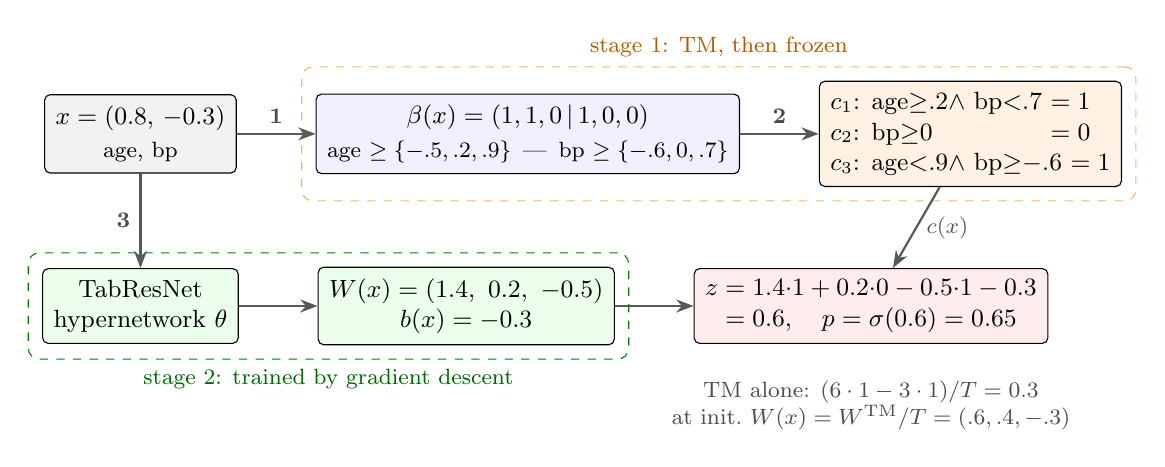
\begin{tikzpicture}[
    font=\small, >={Stealth[length=2.2mm]},
    box/.style={draw, rounded corners=2pt, align=center, inner sep=4pt, fill=#1},
    box/.default=white,
    lab/.style={font=\footnotesize\bfseries, text=black!70},
    arr/.style={->, thick, black!65}]
  % column 1: input
  \node[box=gray!10, minimum width=2.3cm] (x) {$x=(0.8,\,-0.3)$\\[1pt]\footnotesize age, bp};
  % column 2: bits
  \node[box=blue!6, right=1.0cm of x, minimum width=3.1cm] (bits)
    {$\beta(x)=(1,1,0\,|\,1,0,0)$\\[1pt]\footnotesize age $\ge\{-.5,.2,.9\}$ \,|\, bp $\ge\{-.6,0,.7\}$};
  % column 3: clauses
  \node[box=orange!10, right=1.0cm of bits, align=left] (cl)
    {$c_1$: age${\ge}.2\land$ bp${<}.7$ \hfill $=1$\\
     $c_2$: bp${\ge}0$ \hfill $=0$\\
     $c_3$: age${<}.9\land$ bp${\ge}{-.6}$ \hfill $=1$};
  % hypernetwork below
  \node[box=green!8, below=1.2cm of x, minimum width=2.3cm] (hn) {TabResNet\\hypernetwork $\theta$};
  \node[box=green!8, right=1.0cm of hn, minimum width=3.1cm] (w)
    {$W(x)=(1.4,\ 0.2,\ -0.5)$\\$b(x)=-0.3$};
  % local model
  \node[box=red!7, right=1.0cm of w, align=center] (z)
    {$z=1.4{\cdot}1+0.2{\cdot}0-0.5{\cdot}1-0.3$\\$=0.6,\quad p=\sigma(0.6)=0.65$};
  \draw[arr] (x) -- node[above, lab]{1} (bits);
  \draw[arr] (bits) -- node[above, lab]{2} (cl);
  \draw[arr] (x) -- node[left, lab]{3} (hn);
  \draw[arr] (hn) -- (w);
  \draw[arr] (w) -- (z);
  \draw[arr] (cl) -- node[right, font=\footnotesize]{$c(x)$} (z);
  % stage annotations
  \begin{scope}[on background layer]
    \node[draw=orange!60, dashed, rounded corners, fit=(bits)(cl), inner sep=5pt,
          label={[font=\footnotesize, text=orange!70!black]above:stage 1: TM, then frozen}] {};
    \node[draw=green!50!black, dashed, rounded corners, fit=(hn)(w), inner sep=5pt,
          label={[font=\footnotesize, text=green!40!black]below:stage 2: trained by gradient descent}] {};
  \end{scope}
  \node[below=0.35cm of z, align=center, font=\footnotesize, text=black!70]
    {TM alone: $(6\cdot1-3\cdot1)/T=0.3$\\ at init.\ $W(x)=W^\text{TM}/T=(.6,.4,-.3)$};
\end{tikzpicture}
\caption{\textbf{The worked example of Section~\ref{sec:example}.} (1) The standardised input is cut at
training-set thresholds into bits. (2) The frozen TM clauses are evaluated on the bits. (3) Separately,
the hypernetwork maps the raw input to one weight per clause plus a bias. The logit is the sum of the
weights of the active clauses ($c_j=1$). Only the hypernetwork is trained in stage~2. Numbers are
illustrative.}
\label{fig:worked}
\end{figure}


\section{Experimental protocol}\label{sec:protocol}
\paragraph{Data.} Tier~1 is 12 of the paper's 35 AutoML-benchmark datasets (5--145 features, 690--48,842
rows, 3 multi-class); Tier~2 the other 23. Preprocessing follows the official code (standardisation, target
encoding for binary and ordinal encoding for multi-class tasks). Every method sees the same stratified
60/20/20 train/validation/test split per seed; the TM needs a validation split, and giving it to all
methods keeps the comparison fair, but it also means our numbers are not directly comparable to the
paper's 80/20 protocol.
\paragraph{Methods.} LR, DT, RF (500 trees), GBDT (sklearn HistGradientBoosting; CatBoost was unavailable),
TabResNet, \imn{}, TM, and the TM-based arms of Section~\ref{sec:method}.
\paragraph{Statistics.} The unit of analysis is the dataset-level mean test AUROC over seeds. We report
average ranks with a Friedman test and Nemenyi critical difference (as in the paper) and preregistered
two-sided Wilcoxon signed-rank tests with Holm correction, plus a paired bootstrap CI of the mean
difference. Non-inferiority of \arm{IMN-TM} to \imn{} was preregistered as a 95\% CI above $-0.01$.
\paragraph{Rules.} The library was not modified; every number is generated from the run records; all
selection uses validation data only. Deviations from the paper are logged in \texttt{DECISIONS.md}.

\section{Results}
\subsection{Phase 1: regulariser of the clause arms}\label{sec:reg}
\begin{table}[h]
  \centering\small
  \caption{Mean validation AUROC over 6 datasets $\times$ 3 seeds (\RegRecords{} runs) for the nine
  penalty settings. The selected setting is \texttt{\RegMode}, $\lambda=\RegLambda$.}
  \label{tab:reg}
  \begin{tabular}{lcc}
\toprule
$\ell_1$ mode, $\lambda$ & IMN-TM & IMN-Hybrid \\
\midrule
\texttt{prior}, 1 & 0.8508 & 0.8510 \\
\texttt{all}, 1 & 0.8485 & 0.8501 \\
\texttt{all}, 0.1 & 0.8461 & 0.8454 \\
\texttt{active}, 1 & 0.8456 & 0.8464 \\
\texttt{prior}, 0.1 & 0.8456 & 0.8454 \\
\texttt{prior}, 0.01 & 0.8440 & 0.8442 \\
\texttt{active}, 0.1 & 0.8438 & 0.8447 \\
\texttt{all}, 0.01 & 0.8433 & 0.8454 \\
\texttt{active}, 0.01 & 0.8425 & 0.8444 \\
\bottomrule
\end{tabular}

\end{table}
Shrinking toward the TM's votes with the largest weight tried wins for both clause arms
(Table~\ref{tab:reg}), but all nine settings lie within a few thousandths of AUROC, and the winner sits at
the edge of the grid; the tuned stage therefore searches $\lambda\in[10^{-5},10]$.

\subsection{Main benchmark, default hyper-parameters}\label{sec:main}
\begin{table}[t]
  \centering
  \caption{Test AUROC (mean{\tiny$\pm$sd} over \MainSeeds{} seeds), default hyper-parameters. Top: baselines;
  bottom: TM family, with \imn{} repeated for reference. Bold: best within each half. Last column: the paper's
  Table~8 \imn{} value (its own split; reference only).}
  \label{tab:main}
  \small
  \resizebox{\textwidth}{!}{\begin{tabular}{lcccccc}
\toprule
Dataset & LR & DT & RF & GBDT & TabResNet & IMN \\
\midrule
kr-vs-kp & 0.990{\tiny$\pm$0.003} & 0.985{\tiny$\pm$0.003} & 0.998{\tiny$\pm$0.001} & \textbf{1.000{\tiny$\pm$0.000}} & 0.997{\tiny$\pm$0.002} & 0.997{\tiny$\pm$0.002} \\
credit-g & 0.777{\tiny$\pm$0.053} & 0.634{\tiny$\pm$0.046} & 0.798{\tiny$\pm$0.047} & 0.787{\tiny$\pm$0.045} & 0.798{\tiny$\pm$0.047} & \textbf{0.799{\tiny$\pm$0.044}} \\
vehicle & 0.937{\tiny$\pm$0.009} & 0.799{\tiny$\pm$0.016} & 0.929{\tiny$\pm$0.004} & 0.925{\tiny$\pm$0.011} & 0.957{\tiny$\pm$0.007} & \textbf{0.957{\tiny$\pm$0.008}} \\
kc1 & 0.813{\tiny$\pm$0.012} & 0.638{\tiny$\pm$0.044} & \textbf{0.827{\tiny$\pm$0.007}} & 0.797{\tiny$\pm$0.014} & 0.810{\tiny$\pm$0.018} & 0.812{\tiny$\pm$0.005} \\
blood-transfusion & 0.739{\tiny$\pm$0.037} & 0.610{\tiny$\pm$0.042} & 0.665{\tiny$\pm$0.052} & 0.680{\tiny$\pm$0.072} & 0.738{\tiny$\pm$0.052} & \textbf{0.742{\tiny$\pm$0.047}} \\
phoneme & 0.810{\tiny$\pm$0.009} & 0.822{\tiny$\pm$0.017} & \textbf{0.957{\tiny$\pm$0.006}} & 0.950{\tiny$\pm$0.006} & 0.867{\tiny$\pm$0.007} & 0.882{\tiny$\pm$0.005} \\
adult & 0.902{\tiny$\pm$0.003} & 0.753{\tiny$\pm$0.006} & 0.917{\tiny$\pm$0.002} & \textbf{0.927{\tiny$\pm$0.001}} & 0.905{\tiny$\pm$0.003} & 0.904{\tiny$\pm$0.002} \\
Australian & 0.922{\tiny$\pm$0.019} & 0.824{\tiny$\pm$0.039} & \textbf{0.941{\tiny$\pm$0.010}} & 0.932{\tiny$\pm$0.020} & 0.928{\tiny$\pm$0.020} & 0.923{\tiny$\pm$0.022} \\
segment & 0.993{\tiny$\pm$0.002} & 0.981{\tiny$\pm$0.003} & 0.998{\tiny$\pm$0.001} & \textbf{0.999{\tiny$\pm$0.000}} & 0.995{\tiny$\pm$0.001} & 0.995{\tiny$\pm$0.001} \\
jungle\_chess & 0.805{\tiny$\pm$0.003} & 0.798{\tiny$\pm$0.006} & 0.943{\tiny$\pm$0.002} & \textbf{0.974{\tiny$\pm$0.001}} & 0.903{\tiny$\pm$0.008} & 0.917{\tiny$\pm$0.003} \\
jasmine & 0.853{\tiny$\pm$0.009} & 0.749{\tiny$\pm$0.015} & \textbf{0.879{\tiny$\pm$0.006}} & 0.864{\tiny$\pm$0.003} & 0.858{\tiny$\pm$0.011} & 0.859{\tiny$\pm$0.011} \\
sylvine & 0.966{\tiny$\pm$0.003} & 0.913{\tiny$\pm$0.011} & 0.981{\tiny$\pm$0.002} & \textbf{0.984{\tiny$\pm$0.002}} & 0.976{\tiny$\pm$0.003} & 0.977{\tiny$\pm$0.002} \\
\bottomrule
\end{tabular}
}\\[4pt]
  \resizebox{\textwidth}{!}{\begin{tabular}{lcccccccc}
\toprule
Dataset & IMN & TM & Clause-LR & IMN-TM & IMN-TM (rand.) & IMN-Hybrid & TM-Gated & Paper IMN \\
\midrule
kr-vs-kp & 0.997{\tiny$\pm$0.002} & 0.996{\tiny$\pm$0.004} & 0.997{\tiny$\pm$0.002} & 0.998{\tiny$\pm$0.002} & 0.998{\tiny$\pm$0.002} & 0.998{\tiny$\pm$0.002} & \textbf{0.998{\tiny$\pm$0.002}} & 0.999 \\
credit-g & \textbf{0.799{\tiny$\pm$0.044}} & 0.779{\tiny$\pm$0.043} & 0.768{\tiny$\pm$0.040} & 0.777{\tiny$\pm$0.036} & 0.756{\tiny$\pm$0.038} & 0.774{\tiny$\pm$0.035} & 0.754{\tiny$\pm$0.034} & 0.751 \\
vehicle & \textbf{0.957{\tiny$\pm$0.008}} & 0.913{\tiny$\pm$0.020} & 0.919{\tiny$\pm$0.020} & 0.922{\tiny$\pm$0.019} & 0.939{\tiny$\pm$0.011} & 0.926{\tiny$\pm$0.017} & 0.918{\tiny$\pm$0.016} & 0.957 \\
kc1 & 0.812{\tiny$\pm$0.005} & 0.813{\tiny$\pm$0.016} & 0.826{\tiny$\pm$0.008} & 0.831{\tiny$\pm$0.012} & 0.829{\tiny$\pm$0.007} & \textbf{0.834{\tiny$\pm$0.013}} & 0.785{\tiny$\pm$0.012} & 0.805 \\
blood-transfusion & \textbf{0.742{\tiny$\pm$0.047}} & 0.696{\tiny$\pm$0.054} & 0.694{\tiny$\pm$0.069} & 0.698{\tiny$\pm$0.066} & 0.709{\tiny$\pm$0.063} & 0.700{\tiny$\pm$0.064} & 0.681{\tiny$\pm$0.083} & 0.742 \\
phoneme & 0.882{\tiny$\pm$0.005} & 0.918{\tiny$\pm$0.006} & 0.927{\tiny$\pm$0.007} & 0.926{\tiny$\pm$0.007} & 0.917{\tiny$\pm$0.005} & 0.926{\tiny$\pm$0.007} & \textbf{0.935{\tiny$\pm$0.008}} & 0.950 \\
adult & 0.904{\tiny$\pm$0.002} & 0.876{\tiny$\pm$0.003} & 0.887{\tiny$\pm$0.002} & 0.899{\tiny$\pm$0.003} & 0.904{\tiny$\pm$0.002} & 0.900{\tiny$\pm$0.003} & \textbf{0.906{\tiny$\pm$0.002}} & 0.915 \\
Australian & 0.923{\tiny$\pm$0.022} & 0.922{\tiny$\pm$0.019} & 0.934{\tiny$\pm$0.017} & 0.932{\tiny$\pm$0.019} & \textbf{0.935{\tiny$\pm$0.022}} & 0.933{\tiny$\pm$0.021} & 0.926{\tiny$\pm$0.022} & 0.908 \\
segment & 0.995{\tiny$\pm$0.001} & 0.997{\tiny$\pm$0.001} & 0.998{\tiny$\pm$0.000} & 0.998{\tiny$\pm$0.000} & 0.998{\tiny$\pm$0.001} & \textbf{0.998{\tiny$\pm$0.000}} & 0.998{\tiny$\pm$0.001} & 0.994 \\
jungle\_chess & 0.917{\tiny$\pm$0.003} & 0.958{\tiny$\pm$0.003} & 0.965{\tiny$\pm$0.002} & 0.965{\tiny$\pm$0.003} & 0.956{\tiny$\pm$0.003} & 0.965{\tiny$\pm$0.002} & \textbf{0.972{\tiny$\pm$0.002}} & 0.978 \\
jasmine & 0.859{\tiny$\pm$0.011} & 0.846{\tiny$\pm$0.006} & 0.851{\tiny$\pm$0.006} & 0.852{\tiny$\pm$0.012} & \textbf{0.864{\tiny$\pm$0.015}} & 0.850{\tiny$\pm$0.010} & 0.838{\tiny$\pm$0.008} & 0.865 \\
sylvine & 0.977{\tiny$\pm$0.002} & 0.968{\tiny$\pm$0.002} & 0.974{\tiny$\pm$0.003} & 0.972{\tiny$\pm$0.002} & 0.976{\tiny$\pm$0.003} & 0.973{\tiny$\pm$0.002} & \textbf{0.978{\tiny$\pm$0.002}} & 0.981 \\
\bottomrule
\end{tabular}
}
\end{table}
\begin{table}[t]
  \centering\small
  \caption{Preregistered comparisons, default hyper-parameters (\MainDatasets{} datasets).
  $^\ast$: Holm-corrected $p<0.05$.}
  \label{tab:mainpairs}
  \begin{tabular}{llrcccc}
\toprule
Q & Comparison $A$ vs.\ $B$ & mean $A{-}B$ & 95\% bootstrap CI & W/L & $p$ & $p_\text{Holm}$ \\
\midrule
Q1 & IMN-TM vs.\ TM & +0.0074 & [+0.0038, +0.0114] & 11/1 & 0.002 & 0.024$^\ast$ \\
Q2 & IMN-TM vs.\ IMN & +0.0006 & [-0.0140, +0.0160] & 6/6 & 1.000 & 1.000 \\
Q3 & IMN-Hybrid vs.\ IMN & +0.0011 & [-0.0134, +0.0163] & 6/6 & 1.000 & 1.000 \\
Q3 & IMN-Hybrid vs.\ IMN-TM & +0.0005 & [-0.0004, +0.0014] & 9/3 & 0.204 & 1.000 \\
Q4 & TM-Gated vs.\ LR & +0.0151 & [-0.0158, +0.0538] & 7/5 & 0.970 & 1.000 \\
Q4 & TM-Gated vs.\ TM & +0.0004 & [-0.0090, +0.0094] & 8/4 & 0.733 & 1.000 \\
Q4 & TM-Gated vs.\ IMN & -0.0063 & [-0.0250, +0.0134] & 7/5 & 0.850 & 1.000 \\
Q5 & IMN-TM vs.\ Clause-LR & +0.0024 & [+0.0002, +0.0050] & 9/3 & 0.110 & 0.879 \\
Q6 & IMN-TM vs.\ IMN-TM (rand.) & -0.0009 & [-0.0061, +0.0049] & 5/7 & 0.569 & 1.000 \\
R & IMN vs.\ TabResNet & +0.0026 & [-0.0004, +0.0061] & 9/3 & 0.092 & 0.831 \\
\bottomrule
\end{tabular}

\end{table}
Table~\ref{tab:main} gives the per-dataset results and Table~\ref{tab:mainpairs} the preregistered tests.
\begin{itemize}
  \item \textbf{Q1 (vs.\ the TM).} \arm{IMN-TM} improves on its own source TM on \MainimntmtmWins{} of
        \MainDatasets{} datasets (mean \MainimntmtmMean, CI [\MainimntmtmLo, \MainimntmtmHi], Holm
        $p=\MainimntmtmHolm$), the only significant comparison.
  \item \textbf{Q2 (vs.\ \imn).} Mean difference \MainimntmimnMean{} with \MainimntmimnWins/\MainimntmimnLosses{}
        wins/losses; the CI [\MainimntmimnLo, \MainimntmimnHi] is too wide to establish the preregistered
        non-inferiority margin, so the question is open in both directions.
  \item \textbf{Q3--Q6.} The hybrid behaves like \arm{IMN-TM} (\MainimnhybridimntmMean); \arm{TM-Gated} is
        level with LR, the TM and \imn{}; the per-example generator adds \MainimntmclauselrMean{} over a
        global re-fit of the clause weights; random clauses reach the same AUROC as learned ones
        (\MainimntmimntmrandMean).
  \item \textbf{Reproduction.} \imn{} and TabResNet are statistically indistinguishable
        (\MainimntabresnetMean), as in the paper; the largest gaps to the paper's own numbers are
        \MainWorstPaperGap.
\end{itemize}
Average ranks are in Figure~\ref{fig:ranks}: RF (\MainRankrf) and GBDT (\MainRankgbdt) lead; all
mesomorphic variants lie between \MainRankimntmrand{} and \MainRanktmgated{} (Friedman
$p=\MainFriedmanP$, critical difference \MainCD).

\begin{figure}[t]
  \centering
  \begin{subfigure}[t]{0.49\textwidth}\centering
    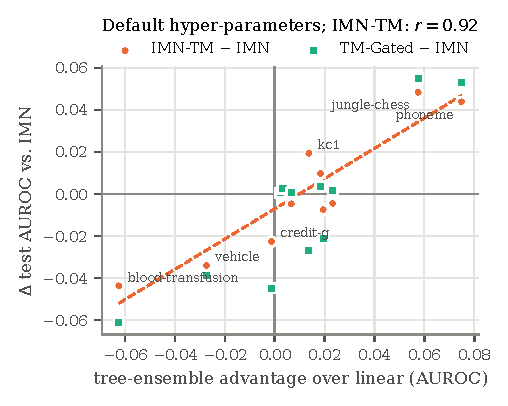
\includegraphics[width=\linewidth]{figures/main_gap.pdf}
    \caption{Gain over \imn{} vs.\ the tree-ensemble advantage over linear models (one point per dataset).}
    \label{fig:gap}
  \end{subfigure}\hfill
  \begin{subfigure}[t]{0.49\textwidth}\centering
    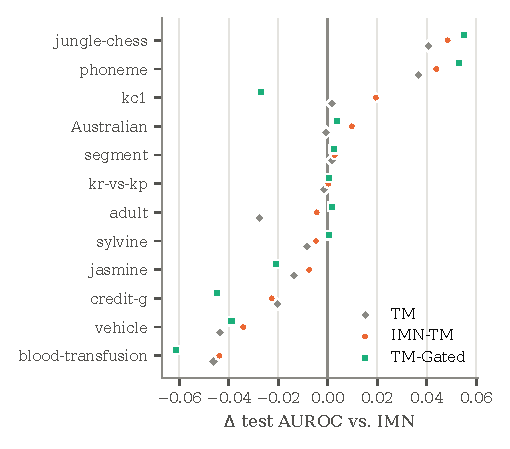
\includegraphics[width=\linewidth]{figures/main_delta.pdf}
    \caption{Per-dataset $\Delta$AUROC vs.\ \imn{}, sorted by the \arm{IMN-TM} gain.}
    \label{fig:delta}
  \end{subfigure}
  \caption{\textbf{Where the TM helps.} Default hyper-parameters, mean over \MainSeeds{} seeds.}
  \label{fig:where}
\end{figure}

\paragraph{The gain is predictable.} The average hides a strong structure (Figure~\ref{fig:where}):
the per-dataset gain of \arm{IMN-TM} over \imn{} correlates with the gap between the best tree ensemble and
the best linear model at $r=\MainGapCorr$. Where axis-aligned thresholds and interactions matter
(phoneme, jungle-chess, kc1), conjunctive local models beat hyperplanes; where the problem is smooth or
nearly linear (blood-transfusion, vehicle, credit-g), they lose. The hybrid was meant to cover both cases
but does not; Section~\ref{sec:abl} tests whether the strong prior penalty suppresses its linear term.

\subsection{Interpretability}\label{sec:interp}
\begin{table}[t]
  \centering\small
  \caption{Explanation size and validity (500 test examples per run, mean over datasets and seeds).
  ``terms'': number of terms covering 90\% of the absolute contribution; self-consist.: cosine between the
  frozen-local-model attribution and the removal effect on the full model; fid.: accuracy of an example's
  local model on its $k$ nearest test neighbours per class.}
  \label{tab:interp}
  \begin{tabular}{lccccccc}
\toprule
Method & lin.\ terms & clause terms & active clauses & literals/clause & self-consist. & fid.\ $k{=}10$ & fid.\ $k{=}50$ \\
\midrule
IMN & 14.9 & -- & -- & -- & 0.649 & 0.553 & 0.581 \\
Clause-LR & -- & 51.8 & 82.6 & 6.7 & 1.000 & 0.736 & 0.777 \\
IMN-TM & -- & 51.0 & 82.6 & 6.7 & 0.965 & 0.724 & 0.764 \\
IMN-TM (rand.) & -- & 40.4 & 79.5 & 4.4 & 0.686 & 0.538 & 0.554 \\
IMN-Hybrid & 9.3 & 50.6 & 82.6 & 6.7 & 0.972 & 0.733 & 0.773 \\
TM-Gated & 16.8 & -- & -- & -- & 0.543 & 0.453 & 0.476 \\
\bottomrule
\end{tabular}

\end{table}
\begin{figure}[t]
  \centering
  \begin{minipage}[b]{0.42\textwidth}\centering
    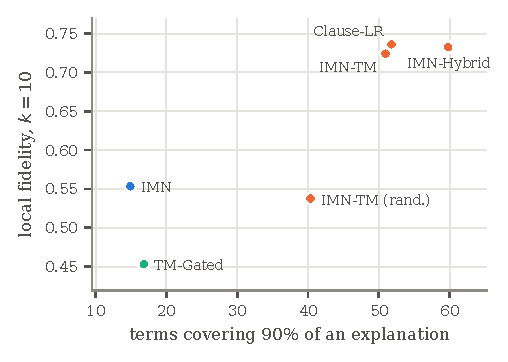
\includegraphics[width=\linewidth]{figures/main_interp.pdf}
    \captionof{figure}{Explanation length vs.\ local fidelity.}
    \label{fig:interp}
  \end{minipage}\hfill
  \begin{minipage}[b]{0.52\textwidth}\centering
    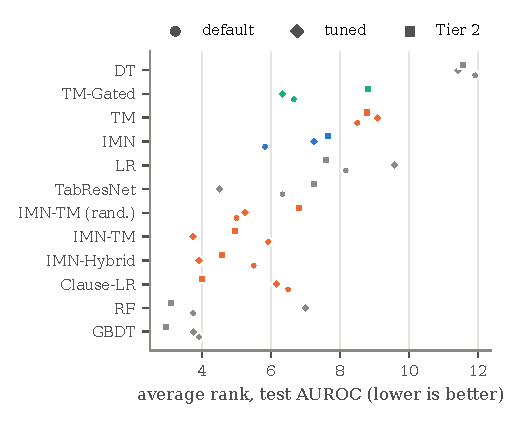
\includegraphics[width=\linewidth]{figures/ranks.pdf}
    \captionof{figure}{Average ranks (test AUROC) per protocol.}
    \label{fig:ranks}
  \end{minipage}
\end{figure}
Clause local models describe the model around an example far better than \imn{}'s hyperplanes
(Table~\ref{tab:interp}, Figure~\ref{fig:interp}): the local model of an example classifies its 10
nearest neighbours per class with accuracy \MainFidimntm{} for \arm{IMN-TM} vs.\ \MainFidimn{} for \imn{},
and the frozen local model agrees with the full model's response to feature removal (self-consistency
\MainSelfimntm{} vs.\ \MainSelfimn). Learned clauses matter here even though they do not matter for
AUROC: random clauses drop to \MainFidimntmrand{} and \MainSelfimntmrand. The cost is length:
\MainClausesimntm{} weighted rules are needed to cover 90\% of an \arm{IMN-TM} explanation vs.\
\MainLinimn{} features for \imn{}. \arm{TM-Gated} gives short linear explanations (\MainLintmgated{} terms) but
the lowest fidelity (\MainFidtmgated): its local hyperplane changes whenever a rule switches.
Figure~\ref{fig:example} shows both kinds of explanation for one real decision.

\begin{figure}[t]
  \centering
  \resizebox{\textwidth}{!}{% generated by code/example_explanation.py -- do not edit
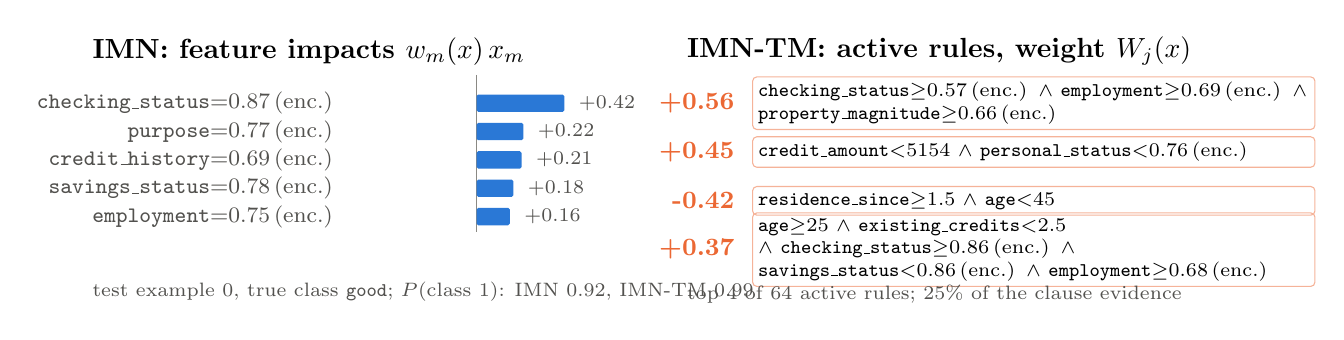
\begin{tikzpicture}[x=1cm,y=1cm,font=\footnotesize]
\node[anchor=west,font=\bfseries] at (0,0.55) {IMN: feature impacts $w_m(x)\,x_m$};
\draw[gaMuted] (5.0,0.25) -- (5.0,-1.75);
\fill[gaBlue,rounded corners=0.6pt] (5.0,0.00) rectangle (6.115,-0.22);
\node[anchor=east,text=gaInkTwo] at (3.3,-0.11) {\texttt{checking\_status}$=$0.87\,(enc.)};
\node[anchor=west,font=\scriptsize,text=gaInkTwo] at (6.175,-0.11) {+0.42};
\fill[gaBlue,rounded corners=0.6pt] (5.0,-0.36) rectangle (5.596,-0.58);
\node[anchor=east,text=gaInkTwo] at (3.3,-0.47) {\texttt{purpose}$=$0.77\,(enc.)};
\node[anchor=west,font=\scriptsize,text=gaInkTwo] at (5.656,-0.47) {+0.22};
\fill[gaBlue,rounded corners=0.6pt] (5.0,-0.72) rectangle (5.573,-0.94);
\node[anchor=east,text=gaInkTwo] at (3.3,-0.83) {\texttt{credit\_history}$=$0.69\,(enc.)};
\node[anchor=west,font=\scriptsize,text=gaInkTwo] at (5.633,-0.83) {+0.21};
\fill[gaBlue,rounded corners=0.6pt] (5.0,-1.08) rectangle (5.467,-1.30);
\node[anchor=east,text=gaInkTwo] at (3.3,-1.19) {\texttt{savings\_status}$=$0.78\,(enc.)};
\node[anchor=west,font=\scriptsize,text=gaInkTwo] at (5.527,-1.19) {+0.18};
\fill[gaBlue,rounded corners=0.6pt] (5.0,-1.44) rectangle (5.424,-1.66);
\node[anchor=east,text=gaInkTwo] at (3.3,-1.55) {\texttt{employment}$=$0.75\,(enc.)};
\node[anchor=west,font=\scriptsize,text=gaInkTwo] at (5.484,-1.55) {+0.16};
\node[anchor=west,font=\bfseries] at (7.55,0.55) {IMN-TM: active rules, weight $W_j(x)$};
\node[anchor=east,text=gaOrange,font=\small\bfseries] at (8.4,-0.11) {+0.56};
\node[anchor=west,draw=gaOrange!50,rounded corners=1.5pt,inner sep=2pt,text width=7.0cm,font=\scriptsize] at (8.5,-0.11) {\texttt{checking\_status}$\ge$0.57\,(enc.) $\wedge$ \texttt{employment}$\ge$0.69\,(enc.) $\wedge$ \texttt{property\_magnitude}$\ge$0.66\,(enc.)};
\node[anchor=east,text=gaOrange,font=\small\bfseries] at (8.4,-0.73) {+0.45};
\node[anchor=west,draw=gaOrange!50,rounded corners=1.5pt,inner sep=2pt,text width=7.0cm,font=\scriptsize] at (8.5,-0.73) {\texttt{credit\_amount}$<$5154 $\wedge$ \texttt{personal\_status}$<$0.76\,(enc.)};
\node[anchor=east,text=gaOrange,font=\small\bfseries] at (8.4,-1.35) {-0.42};
\node[anchor=west,draw=gaOrange!50,rounded corners=1.5pt,inner sep=2pt,text width=7.0cm,font=\scriptsize] at (8.5,-1.35) {\texttt{residence\_since}$\ge$1.5 $\wedge$ \texttt{age}$<$45};
\node[anchor=east,text=gaOrange,font=\small\bfseries] at (8.4,-1.97) {+0.37};
\node[anchor=west,draw=gaOrange!50,rounded corners=1.5pt,inner sep=2pt,text width=7.0cm,font=\scriptsize] at (8.5,-1.97) {\texttt{age}$\ge$25 $\wedge$ \texttt{existing\_credits}$<$2.5 $\wedge$ \texttt{checking\_status}$\ge$0.86\,(enc.) $\wedge$ \texttt{savings\_status}$<$0.86\,(enc.) $\wedge$ \texttt{employment}$\ge$0.68\,(enc.)};
\node[anchor=west,font=\scriptsize,text=gaInkTwo] at (7.55,-2.53) {top 4 of 64 active rules; 25\% of the clause evidence};
\node[anchor=west,font=\scriptsize,text=gaInkTwo] at (0,-2.5) {test example 0, true class \texttt{good}; $P(\text{class 1})$: IMN 0.92, IMN-TM 0.99};
\end{tikzpicture}
}
  \caption{\textbf{One credit-g decision, two explanations} (seed-0 models of Table~\ref{tab:main}).
  Left: \imn{}'s feature impacts. Right: the four strongest of the active rules of \arm{IMN-TM} with their
  per-example weights; thermometer literals of one column are merged into an interval. ``(enc.)'':
  categorical feature in its target-encoded value.}
  \label{fig:example}
\end{figure}

% ---------------------------------------------------------------- remaining phases
% Sections for Phases 3-6; filled in when their records exist.
\subsection{Tuned hyper-parameters}\label{sec:hpo}
Every method received 20 random-search trials per dataset (\S\ref{sec:protocol}). The winner of
each method and dataset was chosen on the seed-0 validation AUROC only and then re-run on
seeds 0--4. Tables~\ref{tab:hpo} and~\ref{tab:hpopairs} repeat the main-stage analysis on these
\HpoRecords{} runs.

\begin{table}[t]
  \centering
  \caption{Test AUROC (mean{\tiny$\pm$sd} over \HpoSeeds{} seeds) with tuned hyper-parameters.
  Layout as in Table~\ref{tab:main}.}
  \label{tab:hpo}
  \small
  \resizebox{\textwidth}{!}{\begin{tabular}{lcccccc}
\toprule
Dataset & LR & DT & RF & GBDT & TabResNet & IMN \\
\midrule
kr-vs-kp & 0.994{\tiny$\pm$0.002} & 0.995{\tiny$\pm$0.002} & 0.995{\tiny$\pm$0.002} & \textbf{0.999{\tiny$\pm$0.000}} & 0.999{\tiny$\pm$0.001} & 0.999{\tiny$\pm$0.001} \\
credit-g & 0.788{\tiny$\pm$0.052} & 0.716{\tiny$\pm$0.052} & 0.794{\tiny$\pm$0.052} & 0.789{\tiny$\pm$0.057} & \textbf{0.796{\tiny$\pm$0.048}} & 0.791{\tiny$\pm$0.045} \\
vehicle & 0.944{\tiny$\pm$0.009} & 0.854{\tiny$\pm$0.018} & 0.925{\tiny$\pm$0.005} & 0.924{\tiny$\pm$0.011} & \textbf{0.958{\tiny$\pm$0.007}} & 0.953{\tiny$\pm$0.011} \\
kc1 & 0.811{\tiny$\pm$0.013} & 0.749{\tiny$\pm$0.037} & \textbf{0.835{\tiny$\pm$0.007}} & 0.820{\tiny$\pm$0.008} & 0.814{\tiny$\pm$0.012} & 0.813{\tiny$\pm$0.010} \\
blood-transfusion & \textbf{0.737{\tiny$\pm$0.032}} & 0.688{\tiny$\pm$0.048} & 0.699{\tiny$\pm$0.037} & 0.694{\tiny$\pm$0.038} & 0.722{\tiny$\pm$0.054} & 0.669{\tiny$\pm$0.058} \\
phoneme & 0.810{\tiny$\pm$0.009} & 0.869{\tiny$\pm$0.011} & 0.919{\tiny$\pm$0.007} & \textbf{0.954{\tiny$\pm$0.005}} & 0.936{\tiny$\pm$0.005} & 0.944{\tiny$\pm$0.005} \\
adult & 0.902{\tiny$\pm$0.003} & 0.900{\tiny$\pm$0.003} & 0.910{\tiny$\pm$0.003} & \textbf{0.928{\tiny$\pm$0.001}} & 0.914{\tiny$\pm$0.002} & 0.912{\tiny$\pm$0.002} \\
Australian & 0.921{\tiny$\pm$0.003} & 0.921{\tiny$\pm$0.016} & 0.937{\tiny$\pm$0.012} & \textbf{0.943{\tiny$\pm$0.016}} & 0.927{\tiny$\pm$0.020} & 0.920{\tiny$\pm$0.023} \\
segment & 0.995{\tiny$\pm$0.001} & 0.989{\tiny$\pm$0.003} & 0.998{\tiny$\pm$0.001} & \textbf{0.999{\tiny$\pm$0.000}} & 0.998{\tiny$\pm$0.000} & 0.997{\tiny$\pm$0.001} \\
jungle\_chess & 0.803{\tiny$\pm$0.003} & 0.856{\tiny$\pm$0.005} & 0.896{\tiny$\pm$0.003} & 0.977{\tiny$\pm$0.001} & \textbf{0.981{\tiny$\pm$0.001}} & 0.980{\tiny$\pm$0.001} \\
jasmine & 0.854{\tiny$\pm$0.008} & 0.838{\tiny$\pm$0.007} & \textbf{0.871{\tiny$\pm$0.005}} & 0.866{\tiny$\pm$0.009} & 0.865{\tiny$\pm$0.009} & 0.861{\tiny$\pm$0.012} \\
sylvine & 0.966{\tiny$\pm$0.003} & 0.957{\tiny$\pm$0.009} & 0.975{\tiny$\pm$0.001} & \textbf{0.985{\tiny$\pm$0.002}} & 0.980{\tiny$\pm$0.003} & 0.977{\tiny$\pm$0.002} \\
\bottomrule
\end{tabular}
}\\[4pt]
  \resizebox{\textwidth}{!}{\begin{tabular}{lcccccccc}
\toprule
Dataset & IMN & TM & Clause-LR & IMN-TM & IMN-TM (rand.) & IMN-Hybrid & TM-Gated & Paper IMN \\
\midrule
kr-vs-kp & 0.999{\tiny$\pm$0.001} & 0.997{\tiny$\pm$0.002} & 0.999{\tiny$\pm$0.001} & \textbf{0.999{\tiny$\pm$0.001}} & \textbf{0.999{\tiny$\pm$0.001}} & 0.999{\tiny$\pm$0.001} & 0.998{\tiny$\pm$0.001} & 0.999 \\
credit-g & 0.791{\tiny$\pm$0.045} & 0.792{\tiny$\pm$0.051} & 0.793{\tiny$\pm$0.051} & 0.799{\tiny$\pm$0.049} & 0.792{\tiny$\pm$0.061} & \textbf{0.799{\tiny$\pm$0.049}} & 0.766{\tiny$\pm$0.030} & 0.751 \\
vehicle & \textbf{0.953{\tiny$\pm$0.011}} & 0.922{\tiny$\pm$0.009} & 0.927{\tiny$\pm$0.008} & 0.936{\tiny$\pm$0.011} & 0.937{\tiny$\pm$0.005} & 0.937{\tiny$\pm$0.011} & 0.931{\tiny$\pm$0.010} & 0.957 \\
kc1 & 0.813{\tiny$\pm$0.010} & 0.804{\tiny$\pm$0.013} & 0.816{\tiny$\pm$0.007} & 0.816{\tiny$\pm$0.008} & 0.817{\tiny$\pm$0.010} & \textbf{0.818{\tiny$\pm$0.009}} & 0.815{\tiny$\pm$0.015} & 0.805 \\
blood-transfusion & 0.669{\tiny$\pm$0.058} & 0.698{\tiny$\pm$0.059} & 0.705{\tiny$\pm$0.065} & 0.706{\tiny$\pm$0.065} & \textbf{0.725{\tiny$\pm$0.057}} & 0.708{\tiny$\pm$0.066} & 0.715{\tiny$\pm$0.051} & 0.742 \\
phoneme & 0.944{\tiny$\pm$0.005} & 0.937{\tiny$\pm$0.005} & 0.943{\tiny$\pm$0.004} & 0.948{\tiny$\pm$0.004} & 0.945{\tiny$\pm$0.004} & \textbf{0.948{\tiny$\pm$0.004}} & 0.945{\tiny$\pm$0.004} & 0.950 \\
adult & 0.912{\tiny$\pm$0.002} & 0.905{\tiny$\pm$0.003} & 0.910{\tiny$\pm$0.003} & 0.912{\tiny$\pm$0.002} & 0.910{\tiny$\pm$0.002} & 0.912{\tiny$\pm$0.002} & \textbf{0.913{\tiny$\pm$0.002}} & 0.915 \\
Australian & 0.920{\tiny$\pm$0.023} & 0.924{\tiny$\pm$0.012} & 0.938{\tiny$\pm$0.010} & \textbf{0.939{\tiny$\pm$0.006}} & 0.938{\tiny$\pm$0.013} & 0.939{\tiny$\pm$0.005} & 0.936{\tiny$\pm$0.011} & 0.908 \\
segment & 0.997{\tiny$\pm$0.001} & 0.998{\tiny$\pm$0.001} & \textbf{0.999{\tiny$\pm$0.000}} & 0.998{\tiny$\pm$0.000} & 0.997{\tiny$\pm$0.001} & 0.996{\tiny$\pm$0.002} & 0.998{\tiny$\pm$0.002} & 0.994 \\
jungle\_chess & \textbf{0.980{\tiny$\pm$0.001}} & 0.969{\tiny$\pm$0.001} & 0.974{\tiny$\pm$0.001} & 0.975{\tiny$\pm$0.002} & 0.970{\tiny$\pm$0.001} & 0.975{\tiny$\pm$0.002} & 0.974{\tiny$\pm$0.002} & 0.978 \\
jasmine & 0.861{\tiny$\pm$0.012} & 0.856{\tiny$\pm$0.012} & 0.863{\tiny$\pm$0.008} & \textbf{0.876{\tiny$\pm$0.009}} & 0.869{\tiny$\pm$0.013} & 0.876{\tiny$\pm$0.009} & 0.862{\tiny$\pm$0.009} & 0.865 \\
sylvine & 0.977{\tiny$\pm$0.002} & 0.971{\tiny$\pm$0.005} & 0.976{\tiny$\pm$0.003} & 0.981{\tiny$\pm$0.002} & 0.978{\tiny$\pm$0.003} & \textbf{0.981{\tiny$\pm$0.002}} & 0.979{\tiny$\pm$0.002} & 0.981 \\
\bottomrule
\end{tabular}
}
\end{table}
\begin{table}[t]
  \centering\small
  \caption{Preregistered comparisons, tuned hyper-parameters (\HpoDatasets{} datasets).
  $^\ast$: Holm-corrected $p<0.05$.}
  \label{tab:hpopairs}
  \begin{tabular}{llrcccc}
\toprule
Q & Comparison $A$ vs.\ $B$ & mean $A{-}B$ & 95\% bootstrap CI & W/L & $p$ & $p_\text{Holm}$ \\
\midrule
Q1 & IMN-TM vs.\ TM & +0.0094 & [+0.0065, +0.0125] & 12/0 & \ensuremath{4.9\times 10^{-4}} & 0.005$^\ast$ \\
Q2 & IMN-TM vs.\ IMN & +0.0058 & [-0.0010, +0.0136] & 9/3 & 0.129 & 0.776 \\
Q3 & IMN-Hybrid vs.\ IMN & +0.0059 & [-0.0010, +0.0139] & 8/4 & 0.176 & 0.776 \\
Q3 & IMN-Hybrid vs.\ IMN-TM & +0.0001 & [-0.0004, +0.0006] & 7/5 & 0.380 & 0.904 \\
Q4 & TM-Gated vs.\ LR & +0.0254 & [-0.0031, +0.0629] & 9/3 & 0.301 & 0.904 \\
Q4 & TM-Gated vs.\ TM & +0.0049 & [-0.0016, +0.0096] & 11/1 & 0.034 & 0.239 \\
Q4 & TM-Gated vs.\ IMN & +0.0013 & [-0.0075, +0.0116] & 8/4 & 0.519 & 0.904 \\
Q5 & IMN-TM vs.\ Clause-LR & +0.0036 & [+0.0015, +0.0060] & 10/2 & 0.003 & 0.031$^\ast$ \\
Q6 & IMN-TM vs.\ IMN-TM (rand.) & +0.0007 & [-0.0035, +0.0037] & 8/4 & 0.151 & 0.776 \\
R & IMN vs.\ TabResNet & -0.0061 & [-0.0155, -0.0001] & 1/11 & 0.027 & 0.215 \\
\bottomrule
\end{tabular}

\end{table}
\begin{figure}[t]
  \centering
  \begin{subfigure}[t]{0.49\textwidth}\centering
    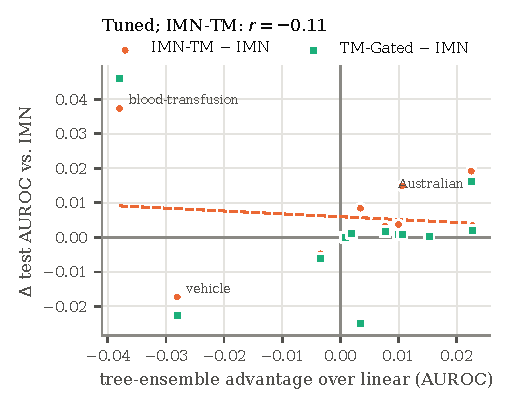
\includegraphics[width=\linewidth]{figures/hpo_final_gap.pdf}
    \caption{Gain over \imn{} vs.\ the tree-ensemble advantage, tuned.}
    \label{fig:hpogap}
  \end{subfigure}\hfill
  \begin{subfigure}[t]{0.49\textwidth}\centering
    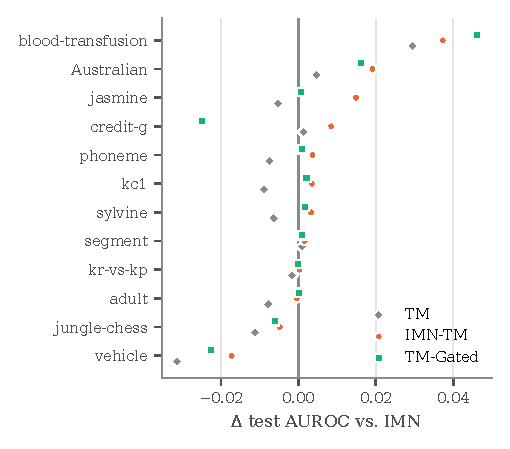
\includegraphics[width=\linewidth]{figures/hpo_final_delta.pdf}
    \caption{Per-dataset $\Delta$AUROC vs.\ \imn{}, tuned.}
    \label{fig:hpodelta}
  \end{subfigure}
  \caption{\textbf{Where the TM helps, after tuning.} Compare with Figure~\ref{fig:where}.}
  \label{fig:hpowhere}
\end{figure}

\paragraph{Tuning helps the clause models most.} \arm{IMN-TM} improves on its default
configuration on \TuneimntmWins{} of 12 datasets (\TuneimntmMean{} mean AUROC, to
\TuneimntmAuroc). \imn{} gains \TuneimnMean{} on \TuneimnWins{} datasets and TabResNet gains
\TunetabresnetMean. Random forests lose \TunerfMean, which shows that selecting on one
validation split is noisy. After tuning, \arm{IMN-TM} shares the best average rank with GBDT
(both \HpoRankimntm; \arm{IMN-Hybrid} \HpoRankimnhybrid, TabResNet \HpoRanktabresnet, \imn{}
\HpoRankimn; Figure~\ref{fig:ranks}). The critical difference is \HpoCD, however, so the leading
group cannot be separated statistically.

\paragraph{Preregistered questions.}
\begin{itemize}
  \item \textbf{Q1} is stronger than with defaults: \arm{IMN-TM} beats its source TM on
        \HpoimntmtmWins/12 datasets (\HpoimntmtmMean, Holm $p=\HpoimntmtmHolm$).
  \item \textbf{Q5} becomes significant. The per-example generator beats a single global re-fit
        of the same clause weights by \HpoimntmclauselrMean{}
        (\HpoimntmclauselrWins/\HpoimntmclauselrLosses, Holm $p=\HpoimntmclauselrHolm$).
  \item \textbf{Q2} moves in favour of \arm{IMN-TM} (\HpoimntmimnMean,
        \HpoimntmimnWins/\HpoimntmimnLosses) but remains unresolved: the confidence interval
        includes zero. One dataset dominates the mean: on \HpoImntmImnBest{} the tuned \imn{}
        lost \TuneimnWorst{} against its own default, a selection failure on a dataset of
        748 rows. Without it the mean difference is \HpoImntmImnMeanNoBest.
  \item \textbf{Q6} is unchanged. Random clauses remain as accurate as learned ones
        (\HpoimntmimntmrandMean).
  \item \textbf{R}: tuned \imn{} falls behind tuned TabResNet (\HpoimntabresnetMean,
        \HpoimntabresnetWins/\HpoimntabresnetLosses, Holm $p=\HpoimntabresnetHolm$). The paper
        reports them level.
\end{itemize}

\paragraph{The default-HP pattern does not survive tuning.} With tuning, \imn{} gains most on
exactly the datasets where clauses had helped: \TuneimnBest. The correlation between the
\arm{IMN-TM} gain and the tree-ensemble advantage falls from $r=\MainGapCorr$ to
$r=\HpoGapCorr$ (Figure~\ref{fig:hpowhere}). The default-HP result should therefore be read as
follows. The clause basis gives the hypernetwork a good inductive bias for threshold-shaped
problems without any search. A tuned hyperplane model closes most of that gap, at a much higher
search cost.

\paragraph{Explanations after tuning.} Local fidelity is unchanged (\arm{IMN-TM}
\HpoFidimntm{} vs.\ \imn{} \HpoFidimn) and self-consistency stays high (\HpoSelfimntm). The tuned
clause models choose weaker L1 penalties, though, and their explanations grow from
\MainClausesimntm{} to \HpoClausesimntm{} rules for 90\% of the evidence. An accuracy-only
search therefore trades away explanation length; a search that also scores explanation size
would need an explicit constraint.
\subsection{Tier 2: twenty larger datasets}\label{sec:tier2}
Tier~2 covers the remaining AutoML-benchmark datasets. They have up to 324k training rows,
up to 4{,}296 features and up to 100 classes. Three are excluded (D25): guillermo and robert
fail OpenML's checksum, and albert cannot be downloaded. The remaining \TiertwoDatasets{}
datasets are run with \TiertwoSeeds{} seeds and default hyper-parameters (\TiertwoRecords{}
runs). All runs completed; \TiertwoSkipped{} were skipped for size.

Two preregistered caps keep the cost bounded (D24):
\begin{itemize}
  \item neural training stops after 50{,}000 steps;
  \item the source TM trains for at most 20 epochs.
\end{itemize}
The step cap binds on \TiertwoCappedN{} of the \TiertwoDatasets{} datasets.
Tables~\ref{tab:t2} and~\ref{tab:t2pairs} report the results.

\begin{table}[t]
  \centering
  \caption{Tier 2: test AUROC (mean{\tiny$\pm$sd} over \TiertwoSeeds{} seeds), default
  hyper-parameters with the step cap. Layout as in Table~\ref{tab:main}.}
  \label{tab:t2}
  \small
  \resizebox{\textwidth}{!}{\begin{tabular}{lcccccc}
\toprule
Dataset & LR & DT & RF & GBDT & TabResNet & IMN \\
\midrule
mfeat-factors & 0.997{\tiny$\pm$0.001} & 0.931{\tiny$\pm$0.017} & 0.998{\tiny$\pm$0.001} & 0.998{\tiny$\pm$0.000} & \textbf{0.999{\tiny$\pm$0.000}} & 0.998{\tiny$\pm$0.000} \\
KDDCup09\_appetency & 0.770{\tiny$\pm$0.009} & 0.527{\tiny$\pm$0.011} & 0.791{\tiny$\pm$0.006} & \textbf{0.807{\tiny$\pm$0.003}} & 0.744{\tiny$\pm$0.011} & 0.759{\tiny$\pm$0.003} \\
airlines & 0.680{\tiny$\pm$0.002} & 0.589{\tiny$\pm$0.001} & 0.693{\tiny$\pm$0.003} & \textbf{0.704{\tiny$\pm$0.002}} & 0.677{\tiny$\pm$0.003} & 0.676{\tiny$\pm$0.004} \\
bank-marketing & 0.904{\tiny$\pm$0.003} & 0.702{\tiny$\pm$0.003} & 0.928{\tiny$\pm$0.004} & \textbf{0.930{\tiny$\pm$0.001}} & 0.904{\tiny$\pm$0.002} & 0.903{\tiny$\pm$0.002} \\
cnae-9 & \textbf{0.995{\tiny$\pm$0.003}} & 0.911{\tiny$\pm$0.004} & 0.993{\tiny$\pm$0.002} & 0.970{\tiny$\pm$0.006} & 0.992{\tiny$\pm$0.004} & 0.983{\tiny$\pm$0.004} \\
nomao & 0.986{\tiny$\pm$0.001} & 0.928{\tiny$\pm$0.004} & 0.993{\tiny$\pm$0.001} & \textbf{0.993{\tiny$\pm$0.001}} & 0.986{\tiny$\pm$0.000} & 0.983{\tiny$\pm$0.001} \\
Amazon\_employee\_access & 0.845{\tiny$\pm$0.012} & 0.645{\tiny$\pm$0.023} & 0.849{\tiny$\pm$0.020} & \textbf{0.857{\tiny$\pm$0.018}} & 0.848{\tiny$\pm$0.010} & 0.847{\tiny$\pm$0.010} \\
higgs & 0.684{\tiny$\pm$0.002} & 0.624{\tiny$\pm$0.001} & 0.799{\tiny$\pm$0.005} & \textbf{0.801{\tiny$\pm$0.004}} & 0.721{\tiny$\pm$0.006} & 0.705{\tiny$\pm$0.004} \\
numerai28.6 & \textbf{0.529{\tiny$\pm$0.002}} & 0.503{\tiny$\pm$0.003} & 0.516{\tiny$\pm$0.006} & 0.523{\tiny$\pm$0.001} & 0.502{\tiny$\pm$0.009} & 0.521{\tiny$\pm$0.007} \\
shuttle & 0.961{\tiny$\pm$0.005} & 0.956{\tiny$\pm$0.043} & \textbf{1.000{\tiny$\pm$0.000}} & 0.578{\tiny$\pm$0.028} & 0.947{\tiny$\pm$0.030} & 0.906{\tiny$\pm$0.031} \\
Fashion-MNIST & 0.981{\tiny$\pm$0.000} & 0.883{\tiny$\pm$0.002} & 0.991{\tiny$\pm$0.000} & \textbf{0.993{\tiny$\pm$0.000}} & 0.985{\tiny$\pm$0.001} & 0.984{\tiny$\pm$0.000} \\
APSFailure & 0.961{\tiny$\pm$0.002} & 0.853{\tiny$\pm$0.007} & 0.991{\tiny$\pm$0.002} & \textbf{0.992{\tiny$\pm$0.002}} & 0.987{\tiny$\pm$0.001} & 0.980{\tiny$\pm$0.006} \\
christine & 0.718{\tiny$\pm$0.009} & 0.636{\tiny$\pm$0.011} & 0.798{\tiny$\pm$0.018} & \textbf{0.811{\tiny$\pm$0.011}} & 0.737{\tiny$\pm$0.008} & 0.767{\tiny$\pm$0.007} \\
MiniBooNE & 0.937{\tiny$\pm$0.001} & 0.866{\tiny$\pm$0.003} & 0.980{\tiny$\pm$0.001} & \textbf{0.983{\tiny$\pm$0.001}} & 0.925{\tiny$\pm$0.006} & 0.907{\tiny$\pm$0.002} \\
riccardo & 0.995{\tiny$\pm$0.002} & 0.837{\tiny$\pm$0.009} & 0.998{\tiny$\pm$0.000} & \textbf{1.000{\tiny$\pm$0.000}} & 0.998{\tiny$\pm$0.001} & 0.998{\tiny$\pm$0.001} \\
dilbert & 0.994{\tiny$\pm$0.000} & 0.868{\tiny$\pm$0.004} & 0.998{\tiny$\pm$0.000} & \textbf{1.000{\tiny$\pm$0.000}} & 0.996{\tiny$\pm$0.000} & 0.996{\tiny$\pm$0.000} \\
fabert & 0.873{\tiny$\pm$0.008} & 0.745{\tiny$\pm$0.009} & \textbf{0.920{\tiny$\pm$0.005}} & 0.907{\tiny$\pm$0.005} & 0.901{\tiny$\pm$0.005} & 0.899{\tiny$\pm$0.006} \\
volkert & 0.889{\tiny$\pm$0.002} & 0.693{\tiny$\pm$0.002} & 0.934{\tiny$\pm$0.001} & \textbf{0.937{\tiny$\pm$0.001}} & 0.878{\tiny$\pm$0.003} & 0.891{\tiny$\pm$0.003} \\
jannis & 0.813{\tiny$\pm$0.002} & 0.607{\tiny$\pm$0.004} & 0.861{\tiny$\pm$0.001} & \textbf{0.868{\tiny$\pm$0.003}} & 0.804{\tiny$\pm$0.002} & 0.816{\tiny$\pm$0.005} \\
helena & 0.859{\tiny$\pm$0.003} & 0.549{\tiny$\pm$0.002} & \textbf{0.864{\tiny$\pm$0.000}} & 0.658{\tiny$\pm$0.007} & 0.849{\tiny$\pm$0.003} & 0.857{\tiny$\pm$0.003} \\
\bottomrule
\end{tabular}
}\\[4pt]
  \resizebox{\textwidth}{!}{\begin{tabular}{lcccccccc}
\toprule
Dataset & IMN & TM & Clause-LR & IMN-TM & IMN-TM (rand.) & IMN-Hybrid & TM-Gated & Paper IMN \\
\midrule
mfeat-factors & 0.998{\tiny$\pm$0.000} & 0.997{\tiny$\pm$0.002} & 0.999{\tiny$\pm$0.001} & 0.998{\tiny$\pm$0.001} & \textbf{0.999{\tiny$\pm$0.001}} & 0.998{\tiny$\pm$0.001} & 0.993{\tiny$\pm$0.001} & 0.999 \\
KDDCup09\_appetency & 0.759{\tiny$\pm$0.003} & 0.751{\tiny$\pm$0.008} & \textbf{0.813{\tiny$\pm$0.002}} & 0.806{\tiny$\pm$0.002} & 0.761{\tiny$\pm$0.034} & 0.808{\tiny$\pm$0.002} & 0.757{\tiny$\pm$0.020} & 0.816 \\
airlines & 0.676{\tiny$\pm$0.004} & 0.658{\tiny$\pm$0.005} & \textbf{0.682{\tiny$\pm$0.002}} & 0.672{\tiny$\pm$0.007} & 0.671{\tiny$\pm$0.014} & 0.673{\tiny$\pm$0.002} & 0.652{\tiny$\pm$0.011} & 0.695 \\
bank-marketing & 0.903{\tiny$\pm$0.002} & 0.890{\tiny$\pm$0.007} & 0.904{\tiny$\pm$0.005} & 0.901{\tiny$\pm$0.005} & 0.901{\tiny$\pm$0.004} & 0.903{\tiny$\pm$0.005} & \textbf{0.909{\tiny$\pm$0.004}} & 0.930 \\
cnae-9 & 0.983{\tiny$\pm$0.004} & 0.987{\tiny$\pm$0.005} & 0.996{\tiny$\pm$0.001} & \textbf{0.996{\tiny$\pm$0.002}} & 0.975{\tiny$\pm$0.006} & 0.987{\tiny$\pm$0.005} & 0.967{\tiny$\pm$0.006} & 0.994 \\
nomao & 0.983{\tiny$\pm$0.001} & 0.985{\tiny$\pm$0.001} & 0.989{\tiny$\pm$0.000} & 0.989{\tiny$\pm$0.001} & 0.987{\tiny$\pm$0.001} & 0.989{\tiny$\pm$0.001} & \textbf{0.990{\tiny$\pm$0.000}} & 0.993 \\
Amazon\_employee\_access & 0.847{\tiny$\pm$0.010} & 0.809{\tiny$\pm$0.014} & \textbf{0.850{\tiny$\pm$0.013}} & 0.844{\tiny$\pm$0.016} & 0.848{\tiny$\pm$0.015} & 0.844{\tiny$\pm$0.016} & 0.843{\tiny$\pm$0.016} & 0.858 \\
higgs & 0.705{\tiny$\pm$0.004} & 0.754{\tiny$\pm$0.004} & \textbf{0.772{\tiny$\pm$0.005}} & 0.765{\tiny$\pm$0.005} & 0.706{\tiny$\pm$0.002} & 0.769{\tiny$\pm$0.005} & 0.752{\tiny$\pm$0.005} & 0.823 \\
numerai28.6 & \textbf{0.521{\tiny$\pm$0.007}} & 0.511{\tiny$\pm$0.006} & 0.520{\tiny$\pm$0.005} & 0.509{\tiny$\pm$0.004} & 0.504{\tiny$\pm$0.011} & 0.510{\tiny$\pm$0.004} & 0.509{\tiny$\pm$0.006} & 0.530 \\
shuttle & 0.906{\tiny$\pm$0.031} & 0.952{\tiny$\pm$0.040} & 0.997{\tiny$\pm$0.001} & 0.998{\tiny$\pm$0.001} & 0.997{\tiny$\pm$0.001} & \textbf{0.999{\tiny$\pm$0.001}} & 0.895{\tiny$\pm$0.102} & 0.993 \\
Fashion-MNIST & 0.984{\tiny$\pm$0.000} & 0.982{\tiny$\pm$0.000} & 0.990{\tiny$\pm$0.000} & \textbf{0.990{\tiny$\pm$0.001}} & 0.985{\tiny$\pm$0.000} & 0.989{\tiny$\pm$0.000} & 0.932{\tiny$\pm$0.004} & 0.992 \\
APSFailure & 0.980{\tiny$\pm$0.006} & 0.981{\tiny$\pm$0.005} & 0.988{\tiny$\pm$0.002} & 0.988{\tiny$\pm$0.003} & 0.983{\tiny$\pm$0.001} & \textbf{0.989{\tiny$\pm$0.002}} & 0.847{\tiny$\pm$0.032} & 0.980 \\
christine & 0.767{\tiny$\pm$0.007} & 0.772{\tiny$\pm$0.009} & 0.768{\tiny$\pm$0.007} & \textbf{0.776{\tiny$\pm$0.009}} & 0.745{\tiny$\pm$0.002} & 0.771{\tiny$\pm$0.007} & 0.775{\tiny$\pm$0.009} & 0.775 \\
MiniBooNE & 0.907{\tiny$\pm$0.002} & 0.977{\tiny$\pm$0.001} & 0.980{\tiny$\pm$0.001} & 0.980{\tiny$\pm$0.001} & 0.942{\tiny$\pm$0.012} & 0.980{\tiny$\pm$0.001} & \textbf{0.981{\tiny$\pm$0.001}} & 0.984 \\
riccardo & 0.998{\tiny$\pm$0.001} & 0.998{\tiny$\pm$0.001} & 0.999{\tiny$\pm$0.001} & 0.999{\tiny$\pm$0.001} & 0.998{\tiny$\pm$0.001} & \textbf{0.999{\tiny$\pm$0.000}} & 0.998{\tiny$\pm$0.001} & 0.998 \\
dilbert & 0.996{\tiny$\pm$0.000} & 0.995{\tiny$\pm$0.001} & 0.998{\tiny$\pm$0.000} & 0.998{\tiny$\pm$0.000} & 0.997{\tiny$\pm$0.001} & \textbf{0.999{\tiny$\pm$0.000}} & 0.994{\tiny$\pm$0.001} & 1.000 \\
fabert & 0.899{\tiny$\pm$0.006} & 0.535{\tiny$\pm$0.008} & 0.581{\tiny$\pm$0.019} & 0.899{\tiny$\pm$0.007} & \textbf{0.900{\tiny$\pm$0.007}} & 0.898{\tiny$\pm$0.011} & 0.866{\tiny$\pm$0.019} & 0.902 \\
volkert & 0.891{\tiny$\pm$0.003} & 0.877{\tiny$\pm$0.004} & 0.915{\tiny$\pm$0.002} & 0.915{\tiny$\pm$0.002} & 0.902{\tiny$\pm$0.001} & \textbf{0.919{\tiny$\pm$0.002}} & 0.824{\tiny$\pm$0.004} & 0.943 \\
jannis & 0.816{\tiny$\pm$0.005} & 0.804{\tiny$\pm$0.001} & 0.847{\tiny$\pm$0.001} & 0.847{\tiny$\pm$0.001} & 0.809{\tiny$\pm$0.002} & \textbf{0.849{\tiny$\pm$0.000}} & 0.791{\tiny$\pm$0.001} & 0.856 \\
helena & 0.857{\tiny$\pm$0.003} & 0.780{\tiny$\pm$0.002} & 0.871{\tiny$\pm$0.001} & 0.870{\tiny$\pm$0.002} & 0.865{\tiny$\pm$0.001} & \textbf{0.871{\tiny$\pm$0.002}} & 0.773{\tiny$\pm$0.002} & 0.865 \\
\bottomrule
\end{tabular}
}
\end{table}
\begin{table}[t]
  \centering\small
  \caption{Preregistered comparisons on Tier 2 (\TiertwoDatasets{} datasets).
  $^\ast$: Holm-corrected $p<0.05$.}
  \label{tab:t2pairs}
  \begin{tabular}{llrcccc}
\toprule
Q & Comparison $A$ vs.\ $B$ & mean $A{-}B$ & 95\% bootstrap CI & W/L & $p$ & $p_\text{Holm}$ \\
\midrule
Q1 & IMN-TM vs.\ TM & +0.0372 & [+0.0126, +0.0772] & 19/1 & \ensuremath{9.5\times 10^{-6}} & \ensuremath{9.5\times 10^{-5}}$^\ast$ \\
Q2 & IMN-TM vs.\ IMN & +0.0183 & [+0.0072, +0.0314] & 15/5 & 0.004 & 0.030$^\ast$ \\
Q3 & IMN-Hybrid vs.\ IMN & +0.0185 & [+0.0071, +0.0319] & 15/5 & 0.003 & 0.025$^\ast$ \\
Q3 & IMN-Hybrid vs.\ IMN-TM & +0.0002 & [-0.0011, +0.0013] & 14/6 & 0.064 & 0.350 \\
Q4 & TM-Gated vs.\ LR & -0.0163 & [-0.0354, +0.0024] & 6/14 & 0.090 & 0.359 \\
Q4 & TM-Gated vs.\ TM & +0.0025 & [-0.0271, +0.0442] & 7/13 & 0.294 & 0.883 \\
Q4 & TM-Gated vs.\ IMN & -0.0164 & [-0.0359, +0.0019] & 5/15 & 0.058 & 0.350 \\
Q5 & IMN-TM vs.\ Clause-LR & +0.0141 & [-0.0035, +0.0470] & 7/13 & 0.312 & 0.883 \\
Q6 & IMN-TM vs.\ IMN-TM (rand.) & +0.0133 & [+0.0058, +0.0216] & 16/4 & \ensuremath{5.9\times 10^{-4}} & 0.005$^\ast$ \\
R & IMN vs.\ TabResNet & -0.0003 & [-0.0069, +0.0059] & 7/13 & 0.648 & 0.883 \\
\bottomrule
\end{tabular}

\end{table}

\paragraph{Headline.} On Tier~2 every clause-based question that was open on Tier~1 comes out
significant:
\begin{itemize}
  \item \arm{IMN-TM} beats its TM on \TiertwoimntmtmWins/\TiertwoDatasets{} datasets
        (\TiertwoimntmtmMean, Holm $p=\TiertwoimntmtmHolm$);
  \item it beats \imn{} on \TiertwoimntmimnWins/\TiertwoDatasets{} (\TiertwoimntmimnMean,
        Holm $p=\TiertwoimntmimnHolm$);
  \item learned clauses beat random ones (\TiertwoimntmimntmrandMean,
        \TiertwoimntmimntmrandWins/\TiertwoimntmimntmrandLosses, Holm
        $p=\TiertwoimntmimntmrandHolm$).
\end{itemize}

\paragraph{Most of the gain comes from an under-trained \imn{}.} Our \imn{} falls well short
of the paper's own numbers (Table~\ref{tab:t2}, last column) on \TiertwoShortN{} datasets:
\TiertwoShortList. All \TiertwoShortCapped{} of them are datasets where the step cap stopped
training early. They are also the datasets with the largest \arm{IMN-TM} gains. Across
datasets, the \arm{IMN-TM}$-$\imn{} difference correlates with \imn{}'s shortfall against the
paper at $r=\TiertwoPaperGapCorr$.

The likely mechanism is the initialisation. \arm{IMN-TM} starts from a trained TM's votes, so
a truncated schedule costs it little. \imn{} starts from scratch and loses most of its cosine
schedule.

On the other \TiertwoRestN{} datasets the advantage is \TiertwoRestMean{}
(\TiertwoRestWins/\TiertwoRestLosses, Wilcoxon $p=\TiertwoRestP$). This is the same
small, non-significant edge as on Tier~1 (\S\ref{sec:main}, \S\ref{sec:hpo}). The Tier-2
result is therefore evidence that \arm{IMN-TM} is the better choice \emph{under a fixed
training budget}. It is not evidence that the clause basis is a better local model.

The learned-vs-random gap (Q6) has the same caveat: random clauses give a weaker starting
point.

\paragraph{Other observations.}
\begin{itemize}
  \item \textbf{Clause-LR.} A single global re-fit of the clause weights ranks third
        (\TiertwoRankclauselr). It is ahead of both mesomorphic clause models
        (\arm{IMN-Hybrid} \TiertwoRankimnhybrid, \arm{IMN-TM} \TiertwoRankimntm) and far ahead
        of \imn{} (\TiertwoRankimn). On large datasets, a fixed linear model over trained
        clauses is a strong and cheap interpretable baseline.
  \item \textbf{Leaders.} GBDT (\TiertwoRankgbdt) and RF (\TiertwoRankrf) lead (Friedman
        $p=\TiertwoFriedmanP$, CD \TiertwoCD).
  \item \textbf{Explanation length.} On these wider inputs, an \imn{} explanation needs
        \TiertwoLinimn{} features for 90\% of its evidence, and an \arm{IMN-TM} explanation
        \TiertwoClausesimntm{} clauses.
  \item \textbf{Local fidelity.} \arm{IMN-TM} \TiertwoFidimntm{} vs.\ \imn{} \TiertwoFidimn.
\end{itemize}
\subsection{Synthetic attribution benchmark}\label{sec:xai}
On real data the true reason for a decision is unknown. Phase~4 therefore uses three synthetic
families whose per-feature contributions are known by construction. Each has $d=8$ features
and $n=10{,}000$ examples:
\begin{itemize}
  \item Gaussian linear;
  \item non-linear additive;
  \item piecewise constant, i.e.\ axis-aligned thresholds.
\end{itemize}
Each family is generated at feature correlations $\rho\in\{0, 0.25, 0.5, 0.75\}$ with five
seeds, giving 60 tasks and \XaiRecords{} runs. Every method is explained with the same removal
attribution (\S\ref{sec:method}) on 500 test rows. The headline metric is the Pearson
correlation between these attributions and the true contributions (``GT corr.'',
Table~\ref{tab:xai}, Figure~\ref{fig:xai}).

\begin{table}[t]
  \centering\small
  \caption{Synthetic attribution benchmark: mean over $\rho$ and seeds, per family. GT corr.:
  correlation of the removal attributions with the true contributions. infid.: infidelity
  under small Gaussian perturbations. It penalises piecewise-constant models, whose output
  jumps, and is reported for completeness only.}
  \label{tab:xai}
  \resizebox{\textwidth}{!}{\begin{tabular}{lccccccccc}
\toprule
 & \multicolumn{3}{c}{Gaussian linear} & \multicolumn{3}{c}{Non-linear additive} & \multicolumn{3}{c}{Piecewise constant} \\
\cmidrule(lr){2-4}\cmidrule(lr){5-7}\cmidrule(lr){8-10}
Method & AUROC & GT corr.\ $\uparrow$ & infid.\ $\downarrow$ & AUROC & GT corr.\ $\uparrow$ & infid.\ $\downarrow$ & AUROC & GT corr.\ $\uparrow$ & infid.\ $\downarrow$ \\
\midrule
LR & 0.997 & 0.975 & 2.581 & 0.741 & 0.523 & 0.034 & 0.757 & 0.576 & 0.037 \\
GBDT & 0.990 & 0.934 & 1.026 & 0.984 & 0.612 & 0.960 & 0.990 & 0.638 & 4.512 \\
TabResNet & 0.997 & 0.972 & 0.617 & 0.970 & 0.656 & 0.221 & 0.847 & 0.607 & 0.060 \\
IMN & 0.997 & 0.843 & 0.245 & 0.968 & 0.541 & 0.188 & 0.848 & 0.570 & 0.057 \\
TM & 0.983 & 0.826 & 0.342 & 0.969 & 0.518 & 0.488 & 0.939 & 0.558 & 0.617 \\
Clause-LR & 0.987 & 0.939 & 1.441 & 0.976 & 0.578 & 1.883 & 0.947 & 0.625 & 1.732 \\
IMN-TM & 0.990 & 0.919 & 2.086 & 0.974 & 0.570 & 2.440 & 0.944 & 0.616 & 1.993 \\
IMN-Hybrid & 0.990 & 0.945 & 2.200 & 0.975 & 0.572 & 2.444 & 0.945 & 0.620 & 1.980 \\
TM-Gated & 0.989 & 0.736 & 0.827 & 0.978 & 0.400 & 1.366 & 0.948 & 0.229 & 1.698 \\
\bottomrule
\end{tabular}
}
\end{table}
\begin{figure}[t]
  \centering
  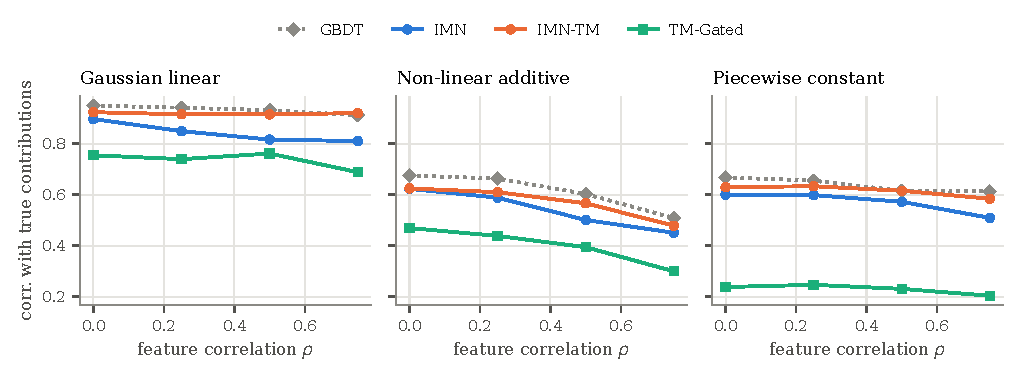
\includegraphics[width=\textwidth]{figures/xai_gt.pdf}
  \caption{\textbf{Attribution quality vs.\ feature correlation.} Mean over five seeds.}
  \label{fig:xai}
\end{figure}

\paragraph{IMN-TM explanations are closer to the truth than \imn{}'s.} Paired over the 60
tasks, the attributions of \arm{IMN-TM} correlate better with the true contributions than those
of \imn{} on \XaiVsimnWins{} of \XaiVsimnN{} tasks (mean \XaiVsimnMean, Wilcoxon
$p=\XaiVsimnP$).
\begin{itemize}
  \item \textbf{Piecewise constant.} The difference is clearest here: \Xaiimntmpiecewise{} for
        \arm{IMN-TM} vs.\ \Xaiimnpiecewise{} for \imn{}. In this family \imn{} is also less
        accurate (AUROC \XaiAucimnpiecewise{} vs.\ \XaiAucimntmpiecewise).
  \item \textbf{Gaussian linear.} Surprisingly, the difference also holds on the linear family
        (\Xaiimntmlinear{} vs.\ \Xaiimnlinear). As $\rho$ rises from 0 to 0.75, \imn{}'s
        correlation drops by \XaiLinDropimn{} and \arm{IMN-TM}'s by only \XaiLinDropimntm.
        With correlated inputs, a per-example hyperplane can shift weight between correlated
        features without changing its output. The TM-initialised clause weights are anchored
        to a global rule set and drift less.
\end{itemize}

\paragraph{Baselines.} The best global models remain ahead.
\begin{itemize}
  \item Plain logistic regression is nearly perfect on its own family (\Xailrlinear).
  \item GBDT's removal attributions beat \arm{IMN-TM} on \XaiVsgbdtLosses{} of the
        \XaiVsgbdtN{} tasks (\XaiVsgbdtMean, $p=\XaiVsgbdtP$).
\end{itemize}
The mesomorphic models are thus not more faithful than a removal-attributed tree ensemble.
Their advantage is that the explanation is the model's own local function, not a post-hoc
probe.

\paragraph{TM-Gated explanations are unreliable.} \arm{TM-Gated} is the least faithful method
in every family (\Xaitmgatedpiecewise{} on piecewise data; \arm{IMN-TM} is ahead on
\XaiVstmgatedWins/\XaiVstmgatedN{} tasks). Its local hyperplane is re-composed from rule-gated
pieces, and the removal of one feature switches rules on or off. The same failure appeared as
low local fidelity on real data (\S\ref{sec:interp}).
\subsection{Ablations}\label{sec:abl}
Each variant of Table~\ref{tab:abl} is run on the twelve Tier-1 datasets with seeds 0--2. It is
compared with the main-stage record of its reference arm on the same seeds, using a paired
Wilcoxon test over datasets without multiplicity correction. No variant changes test AUROC
significantly. Read together, the rows answer four design questions.

\paragraph{Basis size.} The source TM gains from more clauses (800 per class:
\AblTmEightMean, \AblTmEightWins/\AblTmEightLosses{} wins/losses, $p=\AblTmEightP$). IMN-TM
does not (\AblImntmEightMean, $p=\AblImntmEightP$), and 50 clauses per class are also enough
(\AblImntmFiftyMean, $p=\AblImntmFiftyP$). Re-weighting the clauses per example therefore
recovers what a larger TM gets by adding clauses, and the default of 200 is not a binding choice.

\paragraph{Initialisation.} Starting the generated weights at zero instead of at the TM's own
votes leaves accuracy unchanged (\AblNoinitMean, $p=\AblNoinitP$). It does lower local fidelity
from \AblNoinitRefFid{} to \AblNoinitFid. The initialisation is therefore an interpretability
device: it keeps the per-example weights close to a global rule set.

\paragraph{Generator input.} Feeding the clause outputs to the hypernetwork as well,
$[x, c(x)]$, is the worst variant (\AblXcMean, \AblXcWins/\AblXcLosses, $p=\AblXcP$). The
generator then sees the same binary evidence it is weighting, which appears to encourage
over-fitting. The raw input $x$ alone is the better choice.

\paragraph{Which clauses.} Random conjunctions matched to the trained clauses' firing rates give
nearly the same accuracy (\AblRandfrMean, $p=\AblRandfrP$), confirming the main-stage
random-clause control. Their local fidelity, however, drops from \AblRandfrRefFid{} to
\AblRandfrFid. The trained TM is not needed for accuracy, but it is what makes the explanations
generalise to the neighbourhood of an example.

\paragraph{Hybrid split.} Giving the linear block of IMN-Hybrid its own, weaker L1 penalty
($\lambda=0.1$) does not change accuracy (\AblSplitMean, $p=\AblSplitP$). The main-stage
hypothesis that the strong prior penalty suppressed a useful linear term is not supported.

\begin{table}[h]\centering\small
\caption{Ablations (Tier 1, seeds 0--2). $\Delta$ is the test AUROC change versus the reference
arm on the same seeds; $p$ is an uncorrected two-sided Wilcoxon test over datasets. The last
column is local fidelity at $k=10$.}\label{tab:abl}
\begin{tabular}{llcrcccc}
\toprule
Variant & reference & $n$ & mean $\Delta$ & W/L & $p$ & $\Delta$ vs.\ IMN & fid.\ $k{=}10$ \\
\midrule
TM, 50 clauses/class & TM & 12 & -0.0034 & 7/5 & 0.733 & -- & -- \\
TM, 800 clauses/class & TM & 12 & +0.0036 & 9/3 & 0.077 & -- & -- \\
IMN-TM on 50-clause TM & IMN-TM & 12 & +0.0004 & 6/6 & 0.850 & -0.0006 & 0.708 \\
IMN-TM on 800-clause TM & IMN-TM & 12 & -0.0012 & 8/4 & 0.622 & -0.0021 & 0.741 \\
IMN-TM without TM initialisation & IMN-TM & 12 & +0.0002 & 6/6 & 0.970 & -0.0007 & 0.649 \\
IMN-TM, generator input $[x, c(x)]$ & IMN-TM & 12 & -0.0116 & 5/7 & 0.064 & -0.0126 & 0.706 \\
IMN-TM, random clauses (rate-matched) & IMN-TM & 12 & -0.0017 & 8/4 & 0.850 & -0.0026 & 0.557 \\
IMN-Hybrid, linear $\lambda=0.1$ & IMN-Hybrid & 12 & +0.0003 & 8/4 & 0.339 & +0.0001 & 0.738 \\
\bottomrule
\end{tabular}
\end{table}


\FloatBarrier
\section{Limitations}
\begin{itemize}
  \item \textbf{Two-stage training.} The clause basis is fixed before the hypernetwork sees it:
        the TM's clauses are learned for its own fixed vote, not for per-example re-weighting.
        Random clauses match the learned ones in AUROC, so better bases are an open direction.
  \item \textbf{Explanation length.} Clause explanations are long, and an accuracy-only search
        makes them longer. The removal attribution of a clause model depends on the baseline.
  \item \textbf{Hyper-parameter selection.} Winners were selected on one validation split
        (seed 0). On small datasets this is noisy: the tuned \imn{} lost
        \TuneimnWorst{} against its own default.
  \item \textbf{Reproduction.} Our split differs from the paper's. Our default-HP \imn{} falls
        short of the paper's numbers on some datasets (\MainWorstPaperGap), which flatters the
        TM arms there. Tuning closes these gaps.
  \item \textbf{Substitutions and caps.} CatBoost was replaced by HistGradientBoosting. Tier-2
        runs use a step cap that binds on \TiertwoCappedN{} of \TiertwoDatasets{} datasets.
        It favours models with a good initialisation, so Tier-2 differences between \imn{}
        and the clause models partly measure training efficiency
        (Section~\ref{sec:tier2}). Three Tier-2 datasets could not be downloaded verifiably
        and are excluded.
\end{itemize}

\begin{thebibliography}{9}\small
\bibitem{kadra2024} A.~Kadra, S.~Pineda Arango, J.~Grabocka. Interpretable Mesomorphic Networks for Tabular
  Data. \emph{NeurIPS}, 2024.
\bibitem{granmo2018} O.-C.~Granmo. The Tsetlin Machine---A Game Theoretic Bandit Driven Approach to Optimal
  Pattern Recognition with Propositional Logic. \emph{arXiv:1804.01508}, 2018.
\bibitem{xaibench} Y.~Liu, S.~Khandagale, C.~White, W.~Neiswanger. Synthetic Benchmarks for Scientific
  Research in Explainable Machine Learning. \emph{NeurIPS Datasets and Benchmarks}, 2021.
\bibitem{yeh2019} C.-K.~Yeh et al. On the (In)fidelity and Sensitivity of Explanations. \emph{NeurIPS}, 2019.
\end{thebibliography}
\end{document}
